\documentclass[12pt]{article}

\usepackage[onehalfspacing]{setspace}

\usepackage{hyperref}

\usepackage{amsmath}
\usepackage{mathtools}
\usepackage{xfrac}

\usepackage{graphicx}

\usepackage{fancyhdr}
\usepackage{caption}
\usepackage{hhline}
\usepackage{chngpage}
\usepackage{adjustbox}
\usepackage{tabularx}
\usepackage{setspace}
\usepackage{textgreek}
\usepackage{rotating}

\usepackage[backend=bibtex]{biblatex}
\addbibresource{References.bib}

\graphicspath{ {img/} }

\begin{document} 
% h use endash no preceding space

    \begin{titlepage}
    
     \author{
         Tom Bridgwater \and
         Mary O'Donnell \and
         Harapan Ong \and
         Joshua Pegman \and
         Mahera Shaikh \and
         Isabella Sharpley \and
         Alexander Smith \and
         Esther Uwannah \and
         Tim Yau
     }
     
     \title{The Next High Energy Particle Collider}
     
     \maketitle
     \thispagestyle{empty}
     
     \center{
     PHAS3441 - Group 9
          
     Board Member - Dr. Frank Deppisch
     }
    
    \end{titlepage}
 
 \clearpage
 
 \section*{Work Allocation}
\subsection*{Report sections}

\begin{tabularx}{\textwidth}{X r}

    Introduction & Harapan \\
    Executive Summary & Isabella \\
    Basic Particle and Collider Physics & Alexander \& Mary \\
    
    \textbf{Review of Proposed Colliders} & \\
        \hspace{1em} Previous Colliders & Mary \\
        \hspace{1em} ILC & Tim \\
        \hspace{1em} CLIC & Mahera \\
        \hspace{1em} TLEP & Joshua \\
        \hspace{1em} LHeC & Tom \\
        \hspace{1em} Muon-Muon & Harapan \\
        \hspace{1em} SAPPHiRE & Isabella \\        
        
    \textbf{Comparison of ILC and CLIC} & \\
        \hspace{1em} Introduction & Esther \\
        \hspace{1em} Physics Potential & Alexander \& Tom \\
        \hspace{1em} Technological Spin Offs & Mahera \\
        \hspace{1em} Technical Feasibility & Joshua \& Harapan \\
        \hspace{1em} Development Cost & Tim \\
        \hspace{1em} Location \& Governance & Isabella \\
        
    Conclusion & Esther \\    
        

\end{tabularx}

\subsection*{Miscellaneous}

\begin{tabularx}{\textwidth}{X r}

  Chairman & Harapan \\
  Secretary & Esther \& Mahera \\
  Collation, Typesetting and Proofing in Latex & Alexander \& Mary \\
  Review of Group 10 & Alexander \& Joshua \\
  Interviewing Prof. Butterworth, Prof. Waters and Prof. Thorne & Mary \& Harapan \\
  
\end{tabularx}

 
 \clearpage
 
 \setcounter{tocdepth}{2}
 \tableofcontents 
 
 \clearpage
 
 \begin{section}{Introduction}
     On the 4th of July 2012, the European Organisation for Nuclear Research (CERN) announced that the two teams of physicists at the Large Hadron Collider’s (LHC) ATLAS and CMS experiments have discovered a new subatomic particle with a mass of about 126 GeV, which was consistent with the predicted properties of the Higgs boson. The Higgs boson was named after Peter Higgs, who postulated in 1964 the existence of the Higgs field as an explanation for the origin of mass of fundamental particles in the Standard Model (SM) of particle physics. Based on this discovery, the Nobel Prize for Physics 2013 went to Peter Higgs and Francois Englert for the theoretical discovery of the Higgs mechanism, another discovery that served to cement the success of SM physics.
 
Since the discovery of the Higgs boson, research teams around the world have begun proposing what the next stage of particle physics research should be. The general consensus is that with the discovery, more questions and new fields have been opened up for discussion and research, and that these would require a new high energy collider to complement the LHC.
 
While the LHC served its purpose as a “discovery” machine, smashing protons at energies up to 14 TeV, proton-proton collisions produce a large amount of background events that result in “dirty” collisions, which are not ideal conditions for precise measurements of the newly-discovered Higgs boson. These measurements include mass determination, top Yukawa coupling and self-coupling of the Higgs – these measurements require high precision in cleaner collision environments, performed at different energy stages.
 
Besides studying the Higgs mechanism in greater detail, there are still unanswered questions within and beyond SM Physics that physicists hope the next stage in particle physics research can answer. These include gaining a greater insight into the constituents of dark matter and the abundance of matter in our Universe.
 
Hence, the general consensus within the physics community is that the next particle collider to be built needs to be a clean-collision collider (e.g. a lepton collider), capable of performing collisions at different energy stages in order to study different phenomena. Data collected from such a collider would then be the best complement to the experiments that have been run and will run at the LHC.
 
However, such proposals to build another billion-dollar particle collider are not without their critics. Some question the necessity of another particle collider right after the LHC, considering the size and cost of such a project when funding could be channeled to other areas of research in physics.
 \end{section}
 
 \begin{section}{Executive Summary}
 	 The aim of the project was to recommend the best option for the next high energy particle collider with a view to acquiring hypothetical funding for its development. We fulfilled this aim by critically assessing a range of proposed colliders in terms of their physics potential, technical feasibility, technological spin-offs and development cost, while also taking into account the timescale and political aspects of making the project a reality.

The decision making process took into account the following main objectives:

\begin{itemize}
	\item The physics potential of the next collider
    \item The necessary energy reach
    \item Feasibility in terms of technology and time schedule.
    \item What new technology will be produced – spin-offs
    \item Development cost – funding models
    \item Location and governance
    \item Successes and failures of previous particle colliders
\end{itemize}

\subsection{Findings}

The project involved an extensive literature review. We began by evaluating a variety of proposed collider concepts including electron-positron (lepton) colliders, ILC, CLIC and TLeP, a photon collider, SAPPHiRE, the lepton-hadron collider LHeC and muon-muon colliders.

Additionally, a critical assessment of previous colliders was conducted from the 1987 Superconducting Super Collider, which served as a warning about the need for strong political support and adequate funding, to the LHC, which shows the success that can be achieved with a well-planned, well-funded project with a clear science case.

Following the collider evaluations we decided that rather than opt to push the energy barrier, the science community should build a collider that can precisely measure the properties \textendash mass, spin and interaction strengths \textendash of the recently discovered Higgs Boson. Understanding the properties will confirm whether or not this Higgs is that predicted by the Standard Model or instead a link to physics beyond the Standard Model. This in turn will influence the future of particle physics research.

The only way to achieve these measurements is by building a linear lepton collider. The collider must be linear so the energy reach is not be limited by synchrotron radiation. Colliding leptons result in clean collisions and enable us to probe specific energies due to the well-defined centre-of-mass energy.

As well as being the most robust collider proposals of those evaluated, the ILC and CLIC are both linear electron-positron colliders capable of accurately probing the Higgs. As a result we compared them in depth before coming to a well informed decision on the best collider to be built

CLIC presents a higher energy (3 TeV) and luminosity ($10^{35}$ $cm^{-2} s^{-1}$) than the ILC which will have a maximum energy of 1TeV and ten times smaller luminosity $\sim10^{34} cm^{-2} s^{-1}$. Both colliders will be capable of making precise measurements of the Higgs particle, top quark physics and potentially discovering the lightest supersymmetric (SUSY) particles. However CLIC is more viable for the production and observation of the lightest SUSY particles due to its higher energy and luminosity. While the ILC is ready to be built, requiring only industrial scale production of some components, the technology required for CLIC is not ready and requires a further 10 years of R\&D. Also CLIC demands higher running costs due to its 582 MW running power, compared to ILC's 200-250 MW running power requirement. CLIC would be built at CERN according to the conceptual design report and the ILC is likely to be built in Japan (following detailed analysis of potential sites).  

Both machines threw up similar spin-offs which benefit areas of medicine and industry. ILC is much more mature with detailed governance and funding models whereas CLIC is lacking in these respects.

We considered the need for a higher energy reach; accompanying the greater energy reach of CLIC is years of research and development which could be for nothing as the higher energy (14 TeV) LHC may find a particle that requires an even larger energy reach to be examined or indeed find nothing. Therefore why wait to spend 6 billion, building a higher energy machine that would be ran at lower energies. As Professor Butterworth said, ``this is like buying a sports car and only driving it at 30 mph.'' \cite{Butterworth:Interview}

Waiting for higher energy reach is risky and there is a case to be made for building soon \textendash a generation of scientists could go by without building a new collider; consequently there may be no driving force for new physics and a potent economic driver is also lost. On the other hand ILC is ready to go and could be built and running by 2026.

CERN could not cope with running both CLIC and LHC at the same time; it would make particle physics too Europe focused and the power budget of CLIC is too great to operate both simultaneously. In fact the problem of CLIC's enormous power budget has not been solved. The ILC is expected to be hosted by Japan and this provides a good opportunity to internationalise high energy physics through global cooperation.

\subsection{Conclusion}

We concluded that while CLIC would expand the energy frontier, this is not a sufficient reason to choose it over ILC. The science case is not strong enough as there have been no signs of new physics at the LHC and may not be at the higher energy. Therefore the optimal solution is to build the ILC which is more politically and technically feasible and has detailed governance and funding models. The ILC is well motivated to make important measurements like pinning down precision parameters of the Standard Model, the Higgs width and the top couplings; especially given that we know the Higgs is found at 250 GeV and the $t\bar{t}$  at 350 GeV. These measurements need to be made, regardless of whether anything exists at higher energies.

The ILC is well worth the \$7.8 billion development cost and is projected to have a financial impact of $\sim$\$40 billion over a 30 year period while also advancing the quest to explain the fundamental laws of nature and the universe.

Greater detail on the above objectives which lead to our decision to choose the ILC as the next High Energy particle collider is given in the main body of the report along with the accompanying appendices.
 \end{section}

 \begin{section}{Basic Particle and Collider Physics}
      \subsection{Introduction}
 
 Particle colliders are particle accelerators which collide two beams charged particles (e.g. quarks, leptons and bosons) or ionic nuclei into each other or a static target. This is achieved by accelerating the particles with electromagnetic fields to kinetic energies in the regions of giga and tera electron volts (velocities in excess of 0.999c). Well known examples are the Large Hadron Collider (LHC) at CERN and the Tevatron at Fermilab.
 
 \subsection{Collision Physics}
 
 \subsubsection{Lepton vs. Hadron Collisions}
 
 Leptons are elementary particles, whereas hadrons are composed of quarks bound via the strong force. Collisions involving hadrons are actually interactions of the constituent quarks and are modelled as such, however the distribution of energies across the constituent quarks in unknown, so the initial energy of the two colliding particles in a collision is hard to determine. The resulting interactions of hadron-hadron are completely different from lepton-lepton; lepton collisions tend to be considerably cleaner and simpler to analyse, as they are not composite particles and we can accurately know the energies of all particles involved. \cite{CERN:ColliderPhysics}
 
 \subsection{Terms}
 
 \subsubsection{Linear and Circular Colliders}
 
 Colliders can be broken down into two distinct categories, Linear Accelerators (linac) and Circular (ring) Accelerators.
 A linac collides two bunches of particles at a fixed point in the center of a linac. After the collision, the remaining particles can no longer be used since they are travelling in the wrong direction. A ring collider can have multiple collision points along the track (the LHC has four detectors) and after a collision, the uncollided particles continue on to be used again in another collision.  
 
 \subsubsection{Beam Energy}
 
 Collisions are at relativistic speeds so the energy is measured in the center of mass frame.
 
 For a fixed target, the collision energy is proportional to the root of E, whereas two beam energy is proportional to 2E and is therefore more efficient \cite{ITP:Energy}. (See \ref{higherEnergies} for additional information)
 
 \subsubsection{Luminosity}
 
 Luminosity is a representation of the number of events per unit time and is a measure of the colliders performance. Higher luminosity means there is more data available to analyse.
 
 $$
 Luminosity = \frac{n N_1 N_2 f}{A}
 $$
 
 n = number of colliding bunches. $N_{1,2}$ = num of particles in each bunch. f = frequency of collisions. A = cross-sectional area of the beam.
 
 \subsubsection{Synchrotron Radiation}
 
 When charged particles decelerate, they emit their kinetic energy as radiation, this is known as synchrotron radiation (braking radiation or Bremsstrahlung). 
 This detracts from the kinetic energy of the particle and so can impose limits on circular colliders. 
 The amount of energy emitted is inversely proportional to the square of the path radius and proportional to the fourth power of the velocity.  
 Since heavier particles travel slower compared lighter particles with the same kinetic energy, this is a limiting factor for circular colliders of light particles. Accelerating an electron to the same energies as a proton in the LHC would require several orders of magnitude more energy, hence linacs, which do not lose any energy via synchrotron radiation, are often used for light particle collisions.
 
 Synchrotron radiation is used in research as it is the brightest source of artificial X-Rays.
 
 \subsubsection{Acceleration Gradient}
 
 The acceleration gradient is measure of energy imparted on a particle beam per unit length. For a linac, the particle beam only makes one pass and so the acceleration gradient must be very large to reach the required energies. In comparison, ring colliders can accelerate the particles gradually since they may travel around millions of time before collision. This also allows ring colliders to reach energies an order of magnitude higher than linacs before synchrotron losses become prohibitive.
 
 \subsection{Systems}
 \subsubsection{Radiofrequency Cavities}
 
 RF cavities are used to accelerate the particle beam and are typically spaced along the length of collider \cite{CERN:RFCAV}. Electromagnetic waves 
are contained within the cavity and the resulting EM field transfers energy to passing charged particles. The cavities oscillate at a fixed frequency. A particle arriving at exactly the right time will not be subjected to any force, yet ones ahead or behind will be relatively pulled or pushed to match the ideal velocity. This causes particles to bunch into precise groups. On each pass the bunch will increase in energy.

Klystrons produce EM waves which are fed remotely along a metal waveguide to  the RF cavities. An electron beam is bunched via the same method as a RF cavity and then meets an EM wave at a time where the wave opposes the electron's motion, causing the electrons to slow down and transfer energy to the wave. Klystrons operate with a relatively low current, but voltage in the kilovolt region.
 
 \subsubsection{Beam Control}
 
 Aside from the bunching performed by RF cavities, the particle beam needs to be narrowed in the other two planes and, in a ring collider, bent along the path. A quadrupole arrangement of magnets has two north and two south poles at 90 degrees from each other in a circle pattern and is used for focusing the beam like a lens. The field produced has a minimal potential at the center of the beam, forcing stray particles towards the bunch \cite{ILC:BeamFocusing}. Dipole magnets are used to bend particles around the path of a ring collider. 
 
 \subsubsection{Cooling}
 
 Superconductors have an electrical resistance of almost zero. This allows the bending electromagnets to produce extremely strong fields and therefore bend a higher energy particle beam.
 
 Superconducting RF cavities can operate at a higher duty cycle, lower beam impedance (as the apertures can be made wider) and higher efficiency of the RF source (Klystron costs increase exponentially with output). 
 
 The financial savings made from the reduced power requirements during operation is approximately offset by the need to supercool the equipment \cite{ILC:TechnicalDesignReport}.
 
 \subsubsection{Storage Rings and Injectors}
 
Many colliders use a mixture of linacs and rings in a chain to gradually raise the particle energy before the beam reaches the collider. These are referred to as booster or injectors. For example, a ring accelerator can be used to increase the energy of leptons with a low acceleration gradient (before synchrotron losses are a consideration) and then send the bunched particles into a linac for higher energy collisions.

Storage rings hold particles at time dilating speeds, this can be useful to store, filter and bunch slow to produce and/or rapidly decaying particles (e.g. antimatter).

 \subsubsection{Detectors}
  
 Detectors are present at the collision point of the particles to observe their momentum, energy and mass. Typically there are several different detectors, each observing a different property. 
 
 Closest to the collision are the tracking devices, which observe the path of the particles by their interference with matter, similar to a cloud chamber. As charged particles move through the device, electrical signal are picked up and the path is reconstructed by a computer. The momentum of the particle can be deduced from its deflection in a magnetic field.
 
 Calorimeters then detect the energy of particles as they forced to deposit their energy into materials. As different particles interact more strongly with different materials (strong or electroweak), various calorimeters are stacked in layers to detect as many particles as possible.
 
Cherenkov radiation is produced when a particle travels faster than light through a medium and the angle of the radiation is dependent upon the particle's velocity. Detectors with specific mediums can therefore detect the velocity of the particle and when combined with momentum, calculate it's mass. \cite{CERN:Detectors} Additionally, should a charged particle pass through two mediums with different electrical resistances, transition radiation is produced. This is dependent upon the energy of the particle and can help determine it's type.
 
 Muon detectors are the furthest out, as muons are weakly interacting and pass through the other detection layers without interacting and all other particles (except neutrinos) are likely absorbed. Muons displace the electrons from atoms in gas chambers. These free electrons are forced to move to the edge of the detectors by an electric field where they are detected.
 
 \cite{Uni:NuclearNotes} 

     \subsection{Standard Model}
The Standard Model of particle physics is a theoretical framework which describes the interactions of all known fundamental particles via the electromagnetic, weak, and strong interactions. According to our understanding, elementary particles can be divided into quarks and leptons, and further classified according to tiers, or ``generations'', with all stable particles belonging to the first generation. The three fundamental forces described by the Standard Model\textemdash electromagnetism, weak, and strong forces\textemdash are all carried by bosons: massless photons (electromagnetic), massive W and Z bosons (weak), and gluons (strong) \cite{CERN:SM:Online}.

The Standard Model is not a complete theory of fundamental interactions: it is considered to be incompatible with Einstein's theory of general relativity — because general relativity is space-invariant whereas, within the Standard Model, Minkowski space is the fixed background space-time \cite{Colosi:2005:CQG}. We also know from cosmology that the Standard Model accounts for just 4\% of the energy present in the universe — the other 96\% is accounted for by dark matter and dark energy, neither of which is explained by the Standard Model \cite{Krauss:2009:Conference}. Additionally, neutrino oscillation experiments have shown that neutrinos have mass \cite{Fukuda:1998:Kamiokande}, but they are not predicted to have mass by the Standard Model in the same way as other fundamental particles. The Standard Model also fails to account for the observed asymmetry of matter and antimatter in our universe \cite{Sather:1999:MatterA}.

\subsection{Symmetry Breaking}
Symmetry breaking refers to a phenomenon where small changes in a system determine which branch of a bifurcation is taken, thereby deciding the fate of the system. There are two different types of symmetry breaking: explicit symmetry breaking, where ``the dynamical equations are not manifestly invariant under the symmetry group considered'' \cite{Brading:2013:Symmetry}, i.e. the Lagrangian contains terms which break the symmetry under consideration; and spontaneous symmetry breaking, where “solutions exist which are not invariant under the action of this symmetry without any explicit asymmetric input”. This type of symmetry breaking emerged in the study of condensed matter physics, wherein the observation that below the Curie temperature the spins of magnetic dipoles all align in one direction breaks the predicted rotational symmetry for the system \cite{Brading:2013:Symmetry}. The Higgs mechanism by which particles gain mass is one example of spontaneous symmetry breaking in particle physics: below some critical temperature, the electroweak symmetry is broken, and the W and Z bosons acquire masses. Without this spontaneous symmetry breaking via the Higgs mechanism, the W and Z bosons\textemdash which we know experimentally to have mass\textemdash would be predicted as massless, like the photon. \cite{Fermi:Electroweak}

\subsection{CP-violation}
CP-violation is violation of \emph{Charge conjugation Parity symmetry}\textemdash the statement that the laws of physics should be unchanged under the exchange of a particle with its antiparticle. and under the inversion of spatial coordinates. It was proposed after the discovery that the weak interaction breaks parity symmetry, in order to ``restore order'' in the Hilbert space of quantum mechanics. In 1964, clear evidence was presented that weak interactions violated not just C-symmetry or P-symmetry but also the combined CP-symmetry \cite{CroninFitch:CP}. ``Direct'' CP-violation arises mathematically from the Standard Model if there exist at least three generations of quarks.

Since CP-violation can be considered the ``true'' symmetry between particles and antiparticles, CP-violation\textemdash that is, a violation of the symmetries of physical law acting on particles and antiparticles\textemdash could explain the observed asymmetry between quantities of matter and antimatter in the visible universe (in fact, it is generally accepted as a prerequisite, or else the asymmetry between matter and antimatter must have been present at the universe's inception). Since the observed CP-violation in the quark sector of the Standard Model alone does not account for the matter-antimatter asymmetry, CP-violation is also being explored in the lepton sector; alternatively, CP-violation in the Higgs sector could make up the shortfall \cite{LHC:CP:Higgs}.

\subsection{Muon Physics}
Muons ($\mu^{-}$) and muon neutrinos ($\nu_{\mu}$) form the so-called ``second generation'' of leptons. Like the electron, the muon is a spin-$\sfrac{1}{2}$ elementary particle with an electric charge of -1. The muon is approximately 200 times more massive than the electron, weighing in at 105.7 MeV/c$^{2}$ (compared with the electron's 0.511 MeV/c$^{2}$). As a result of its higher mass, the muon does not suffer much Brehmsstralung\textemdash electromagnetic radiation produced by the deceleration of a charged particle when deflected in the electric field of another carged particle\textemdash and consequently synchrotron losses for muons are much smaller than for electrons.

Muons are a viable candidate for a new generation of lepton-lepton colliders due to their large mass relative to the electron\textemdash not only do they suffer less from synchrotron energy losses but the centre-of-mass-energy of the collisions is comparatively higher due to this high rest mass. Like electrons, collisions between muons are ``clean'' as they are fundamental rather than composite particles and do not interact via the strong force. However,  the muon decays via the weak interaction with a mean lifetime of 2.2 \textmu s to an electron and two neutrinos (an electron antineutrino and a muon neutrino, to conserve lepton number). The relatively short lifetime of the muon compared with the electron puts constraints on the ease with which beams of muons can be created, cooled, and collided before the particles decay.

\subsection{Beyond the Standard Model}
\subsubsection{Supersymmetry (SUSY)}
SUSY is a proposed extension of the Standard Model which relates bosons to fermions\textemdash according to SUSY, each particle from the one group has a supersymmetric ‘partner' particle with a spin differing by a half-integer. If SUSY were unbroken, the partners would have identical mass and internal quantum numbers aside from spin; but since no partner particles have yet been discovered for SUSY to be correct it must be a ‘spontaneously broken symmetry'\textemdash that is, the as-yet unobserved ‘superpartners', if they exist, must be more massive than their ‘ordinary' counterparts \cite{CERN:Supersymmetry}. There is some hope that these supersymmetric particles will be observed at the Large Hadron Collider when it starts operating at the 7-14 TeV range; but the observation of a rare decay which would have been even less likely under supersymmetry casts some doubt on the validity of the theory \cite{BBC:SUSY}. According to UCL's Dr Waters, ``it would be surprising if nothing showed up in the 7-14 TeV range, although it may not be SUSY.'' \cite{Waters:Interview}

\subsubsection{Gravity, String Theory, Extra Dimensions}
The Standard Model is generally considered incompatible with general relativity. One proposed extension of the Standard Model is the graviton, a hypothetical elementary particle which mediates the force of gravitation\textemdash in the same way that the W and Z bosons mediate the weak force, gluons mediate the strong force, and photons mediate electromagnetism. As the source of gravitation is the stress-energy tensor, a second-rank tensor, it follows that the graviton must be a spin-2 boson. Like the photon it would have to be massless if it exists, as the gravitational field appears, like electromagnetism, to have unlimited range\textemdash i.e. to be a Yukawa potential (wherein the magnitude of the potential falls off exponentially with the mass of the force-carrying particle, in this case a graviton) with m = 0:

\begin{equation*}
V_\text{Yukawa}(r)= -g^2\frac{e^{-kmr}}{r}
\end{equation*}

Gravitons are predicted by string theory, and may be detectable at the Large Hadron Collider by their absence: according to CERN, ``Collisions in particle accelerators always create balanced events\textemdash just like fireworks\textemdash with particles flying out in all directions. A graviton might escape our detectors, leaving an empty zone that we notice as an imbalance in momentum and energy in the event.'' \cite{CERN:Gravitons:Online,deAquino:Gravitons} It is also typical of extensions of the Standard Model including extra dimensions, such as string theory, to include new particles such as heavy spin-1 particles which could be detected at future particle colliders \cite{CLIC:Concept}.

\subsubsection{Leptoquarks}
Leptoquarks are hypothetical particles which exist in various extensions of the Standard Model and carry both lepton and baryon numbers \cite{PDG:Leptoquark}. Since both quarks and leptons are grouped by pairs into the three generations of matter, the existence of leptoquarks might point to a fundamental symmetry underlying the Standard Model. If leptoquarks exist, they could be created at hadron colliders like the LHC, or at lepton-hadron colliders such as the proposed Large Hadron-electron Collider (LHeC) extension of the LHC \cite{Waters:Interview}. Leptons would couple to quarks\textemdash allowing the violation of conservations of baryon and lepton number (but preserving the difference between baryon and lepton numbers). Between 2003 and 2007 the ZEUS Collaboration searched for first-generation leptoquarks at HERA; however ``no evidence for any leptoquark signal was found,'' \cite{ZEUS:Leptoquark} and according to UCL's Professor Butterworth, ``any physics case based on beyond-the-Standard-Model physics for [a hadron-electron collider] is nonsense.'' \cite{Butterworth:Interview}

 \end{section}
 
 \begin{section}{Review of Proposed Colliders}
 
     \begin{subsection}{Previous Colliders}
        \subsubsection{Hadron Colliders}
Hadron colliders currently have the advantage over lepton colliders of being highest in energy: with muon colliders a subject of ongoing research and development \cite{Fermi:Muon:Online}, all extant and historical lepton colliders have used beams of electrons, which are many orders of magnitude lighter than the proton. Because $m_{p}\gg m_{e}$, the proton has a higher much rest-mass energy and suffers less from synchrotron losses. Hadron colliders are therefore natural ``energy frontier'' machines, with the Large Hadron Collider the latest and arguably most famous example.

There is however a penalty associated with the use of hadrons: because protons are composite particles, comprising a ``sea'' of quarks and gluons, colliding beams of protons results in collisions between the composite partons. As a result, the energies of the collisions are not well-defined: on average, each quark carries $\frac{1}{3}$ of the energy of the proton; in reality collisions take place over an energy spectrum. Without knowing the initial energies of the colliding particles, it is difficult \textendash if not impossible \textendash to use the principle of conservation of energy to calculate the expected masses of the collision products [\ref{interview:butterworth}]. Since protons also interact via the strong force, the uncertainties in the calculations are higher than for weakly-interacting particles like electrons [\ref{interview:butterworth}]. This means that measurements made at hadron machines are inherently less precise than those made at lepton (and lepton-hadron) machines.
\subsubsection{Tevatron}
The Tevatron was a 6.3km $p\overline{p}$ circular accelerator located at Fermilab in Illinois. Its maximum energy was 1 TeV \textendash hence the name. At the time of its construction in 1983, this was the man-made energy frontier. To date, the Tevatron is the second-highest energy machine ever built, surpassed only by the Large Hadron Collider.

\begin{figure}[!htb]
\centering
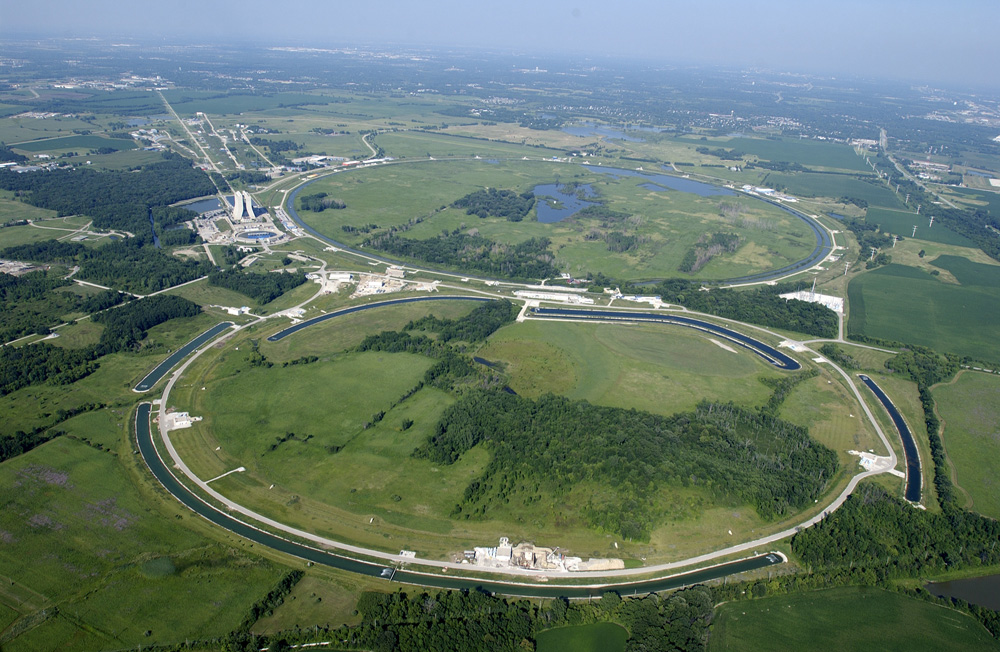
\includegraphics[width=0.7\textwidth,natwidth=1000,natheight=652]{fermilabaccleratorcomplex.jpg}
\caption{Fermilab's Accelerator Complex \cite{Tevatron:Antiprotons:Online}}
\end{figure}

The Tevatron was proposed as a replacement for Fermilab's 500 GeV Main Ring accelerator, which was based on room-temperature electromagnets, and required the development of high-quality superconducting magnets to accelerate the beam, and the design and construction of an antiproton source \cite{Tevatron:Retrospective:Online}. The use of antiprotons allowed the Tevatron to circulate both beams within the same magnet ring (due to the reversed charge on the antiproton), thus saving infrastructure and engineering costs; however, a major limitation to the luminosity of the machine, and therefore the primary focus for upgrades, was the production of antiprotons. The antiprotons used in the Tevatron were produced by ``smashing'' protons into a nickel target, yielding about 20 antiprotons for every $10^{9}$ protons collided with the target \cite{Tevatron:Antiprotons:Online}.

In 1995, the CDF and D\O$\:$ experiments announced the discovery of the top quark, the last fundamental fermion predicted by the Standard Model, with a certainty of 99.9998\% \cite{PhysRevLett:Top1,PhysRevLett:Top2}. Before the completion of the Large Hadron Collider, the Tevatron was the only particle collider energetic enough to produce top quarks. Other discoveries incuded observations of two types of $\sigma$ baryons \cite{Fermi:Sigma:Online}, a $\Xi_{b}^{-}$ baryon \cite{Fermi:Xi:Online}, and a ``double strange'' $\Omega_{b}^{-}$ baryon \cite{PhysRevLett:Omega}. On 2nd July 2012 scientists from the CDF and D\O\: collaborations announced data in support of the existence of a Higgs boson with a mass in the region of 115 to 135 GeV \cite{Fermi:Higgs:Online}; two days later scientists from the LHC announced the discovery of a Higgs with a mass of 125.3 $\pm$ 0.4 (CMS) GeV \cite{PhysLettB:Higgs:CMS} or 126 $\pm$ 0.4 (ATLAS) GeV \cite{PhysLettB:Higgs:ATLAS} \textendash frustratingly, the Higgs boson was so close to the top of the Tevatron's energy range that the Tevatron alone could not furnish proof of its existence.

\subsubsection{Superconducting Super Collider (SSC)}
The Superconducting Super Collider was a proposed proton-proton \cite{SSC:LAT:Online} collider to be built in Texas with a 87.1 km ring circumference. This would have yielded an energy of 20 TeV per proton, and a centre-of-mass-energy of 40 TeV. By comparison, when the Large Hadron Collider reopens in 2015, it will be colliding beams at a centre-of-mass-energy of 13 TeV \cite{LHC:14TeV:Online}. Over 20km worth of tunnel had been excavated and 2,000 on-site staff lost their jobs when the project was cancelled \cite{SSC:Sun:Online}.

\begin{figure}[!htb]
\centering
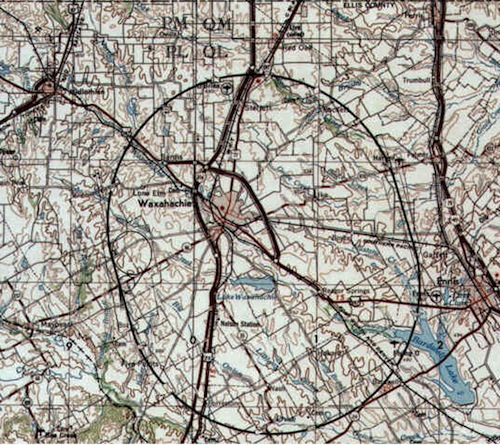
\includegraphics[width=0.7\textwidth,natwidth=500,natheight=445]{sscmap.jpg}
\caption{The SSC was to encircle the town of Waxahachie, Texas \cite{SSC:SI:Online}}
\end{figure}

The reasons for the failure of the Superconducting Super Collider project are many, complex and varied: ultimately budgetary concerns were cited as the reason for cancellation \textendash the United States Congress approved a budget of \$4.4 billion \cite{SSC:BE} for the project in 1987, but cost estimates blew up to over \$11 billion \cite{SSC:LAT:Online} after construction started \textendash however, in large part the project was smothered in its cradle by politics. Prof Steven Weinberg writes:

\begin{quote}
Projected costs did increase, but the main reason was that, year by year, Congress never supplied sufficient funds to keep to the planned rate of spending. This stretched out the time and hence the cost to complete the project. Even so, the SSC met all technical challenges, and could have been completed for about what has been spent on the LHC, and completed a decade earlier. \cite{SSC:Weinberg:Online}
\end{quote}

Prof Jon Butterworth also stated that, ``You can't have it both ways. You've got to either do it as a national project, where you have some helpers, [...] or you do something like CERN where there's no one country in control,'' adding that the decision about whether to fund the International Linear Collider (ILC) as a national prestige project or a collaboration was key to the success of the project [\ref{interview:butterworth}]. The Superconducting Super Collider serves as a cautionary tale about the need for strong political support, and a clear revenue stream.

\subsubsection{Relativistic Heavy Ion Collider (RHIC)}
The Relativistic Heavy Ion Collider (RHIC) is an intersecting storage ring particle accelerator located at the Brookhaven National Laboratory in New York; along with the Large Hadron Collider, which collides ions for one month of the year, it is one of two operational heavy-ion colliders. It is the only spin-polarised proton collider ever built \cite{RHIC:Spin}, which enables it to perform experiments on the spin structure of the proton.

Since the spins of the proton's quarks account for less than one third of its overall spin \cite{PhysLettB:ProtonSpin}, the ``proton spin crisis'' is an important unresolved question in quantum chromodynamics \textendash with potential ramifications for technologies such as Magnetic Resonance Imaging (MRI) \textendash which can be probed by this machine. Notably, the scientists at the RHIC have ``tentatively'' claimed to have created a quark-gluon plasma \cite{NucPhysA:QuarkGluon} \textendash a hypothetical phase of QCD supposed to have existed in the early universe \cite{CERN:QuarkGluonPlasma:Online}. The obvious drawback of the RHIC relative to the LHC is its lower energy \textendash up to around 200 GeV for Au + Au collisions; however, since it runs a dedicated heavy-ion collision programme it outputs more data on the subject compared to the LHC, which collides ions for one month of the year.

\subsubsection{Large Hadron Collider (LHC)}
At 27km in circumference and boasting a centre-of-mass-energy of up to 13 TeV \cite{LHC:14TeV:Online,CERN:14TeV:Online}, the Large Hadron Collider is the largest and most energetic particle collider ever built \cite{LHC:Home}. Located at CERN in Geneva, Switzerland, and crossing the Franco-Swiss border, the Large Hadron Collider is considered ``one of the great engineering milestones of mankind'' \cite{LHC:Milestone:Online}. To date, the great success of the Large Hadron Collider project, and primary reason for funding it, was the discovery of a Higgs boson in 2012 \cite{PhysLettB:Higgs:ATLAS,PhysLettB:Higgs:CMS}. Additionally, the LHC has reported the creation of a quark-gluon plasma \cite{NatGeo:QuarkGluon:Online}, observed the $\chi_{b}$(3P) bottomonium state \cite{arXiv:ATLAS:Bottomonium}, and observed a very rare ($B_{s}^{0} \rightarrow \mu^{+}\mu^{-}$) decay which puts constraints on the likelihood of supersymmetry being correct \cite{BBC:SUSY}. An accident at the LHC in 2008, which involved an electrical fault leading to six tonnes of liquid helium venting into the tunnel and causing an explosion, flags up the importance of stringent failsafes in large-scale experiments. \cite{BBC:MagnetQuench:Online} According to CERN's interim report on the incident: ``Proper safety procedures were in force, safety 
systems performed as expected, and no one was put at risk,'' but the faulty electrics caused an electric arc, which resulted in the explosion \cite{CERN:IncidentReport}.

\begin{figure}[!htb]
\centering
\includegraphics[width=0.7\textwidth,natwidth=1200,natheight=1081]{lhc.jpg}
\caption{The scale of the LHC \cite{ATLAS:Gallery:Online}}
\end{figure}

Due to the low efficiency in the manufacture of antiprotons, the Large Hadron Collider uses colliding beams of protons. The LHC produces data at a rate of tens of petabytes (tens of millions of gigabytes) per year, requiring \textendash by 2012 \textendash the world's largest computer grid, ``a global collaboration of computing centres in nearly 40 countries'', to analyse \cite{LHC:ComputingGrid:Online}.

The Large Hadron Collider is a shining example of the kind of success a well-planned and well-funded large-scale project can achieve; however, it is worth remembering, as Prof Jon Butterworth noted, that ``there was an absolutely first-class science case for the LHC,'' \textendash in other words: it was clear that the Large Hadron Collider was either going to prove or disprove the existence of a Standard Model Higgs, which theoretically had to exist within the energy range accessible at the LHC. This was a clear aim for the project from the outset. However, the lack of additional discoveries \textendash such as supersymmetric particles and dark matter candidates \textendash casts a shadow of doubt over the utility of pushing back the energy barrier further without the theoretical framework to put an upper limit on the mass estimates of these hypothetical particles [\ref{interview:butterworth}]. Additionally, the Large Hadron Collider elided some of the civil engineering costs associated with large particle collider projects because it was built in a pre-existing tunnel (which had previously housed the electron-position collider, LEP) \cite{CERN:LEP:Online}.

\subsubsection{Lepton Colliders}
At present, the only realistic design for a lepton collider utilises beams of electrons (and positrons). The obvious drawback is the small mass of the electron, which places a limit on how energetic the beam can be \textendash particularly for circular colliders, which suffer synchrotron losses. Future designs might use heavier muon or tau particles \cite{Fermi:Muon:Online}, raising the energy ranges available with these colliders.

The particular advantage of a lepton collider is the degree of precision to which measurements can be made, both because leptons are fundamental particles \textendash so the energies of the collisions are well-defined \textendash and because electrons are not subject to the strong force, so the theoretical calculations are also more precise [\ref{interview:thorne}].

\subsubsection{Large Electron-Positron Collider (LEP)}
The Large Electron-Positron Collider, the previous inhabitant of the Large Hadron Collider's 27 km tunnel, was and remains the largest lepton collider ever built. It was completed in 1988, and reached a peak centre-of-mass-energy of 209 GeV \cite{CERN:LEP:Online}. The primary focus of LEP was on measuring the electroweak interaction, and particularly determining the masses of the W and Z bosons, which had been discovered in 1983 (although the most precise measurement of the W mass actually comes from the Tevatron [\ref{interview:butterworth}]). The civil engineering costs associated with building LEP accounted for over half of the construction budget for the machine \cite{LEP:History:Online}. In addition to producing hundreds of thousands of Z bosons \cite{LEP:History:Online}, the machine measured the strength of the strong interaction as decreasing with energy in agreement with quantum chromodynamic theory, and determined the number of particle families with light neutrinos as $2.982\pm 0.013$, in agreement with the Standard Model prediction of 3 \cite{ALEPH:Physics:Online}.

\subsubsection{Lepton-Hadron Colliders}
Lepton-hadron colliders are a``best (and worst) of both worlds'' approach. The use of hadrons means that they can reach higher energies than lepton-only colliders, and the use of leptons means a higher degree of precision than hadron-only colliders. They are particularly good at probing the structure of the proton, and studying quantum chromodynamics (the strong interaction) [\ref{interview:waters}, \ref{interview:thorne}, \ref{interview:butterworth}]. However, they are less energetic than hadron-only machines, and less precise than lepton-only machines.

\subsubsection{Hadron-Elektron Ringanglage (HERA)}
HERA was a 6.3 km particle accelerator located at the Deutsches Elektronen-Synchrotron (DESY) research centre in Hamburg. It collided electrons and positrons with protons at a centre-of-mass-energy of 318 GeV from 1992 to 2007 \cite{PHYS:HERA}. The data obtained at HERA allowed experimenters to obtain the individual parton distribution functions describing the composite nature of the proton and gave ``no indication of a quark substructure down to a scale order of $10^{-18}$m'' \cite{SPS:HERA}, providing strong evidence for the fundamental nature of quarks. HERA measurements also ``confirmed the nature of the strong force as it was predicted by physicists David Gross, David Politzer, and Frank Wilczek'' \cite{PHYS:HERA}. The HERA experiment has been very successful in probing the structure of the proton and testing theoretical models of the strong force; however, any future lepton-hadron collider would necessarily focus on the same area without providing much opportunity to make the kinds of precision measurements available to lepton-only colliders, or push back the energy frontier like a hadron-only collider.
     
     \end{subsection}
     \begin{subsection}{ILC}
         The mission of the International Linear Collider (ILC) is to explore the fundamental composition of nature, i.e. the material and energy constituting the universe, by observing reactions among fundamental particles at the extremely high energy attainable in the superconducting linear collider.
 
\subsubsection{Design}

The electron source for the ILC will use 2 $ns$ laser light pulses to eject electrons from a photocathode, a technique allowing for up to 90\% of the electrons to be polarised; the electrons then will be accelerated to 5 GeV in a 370 meter linac stage. Synchrotron radiation from high energy electrons will produce electron-positron pairs on a titanium-alloy target, with 30\% polarisation; the positrons from these collisions will be collected and accelerated to 5 GeV in a separate linac.
To compact the 5 GeV electron and positron bunches to a sufficiently small size to be usefully collided, they will circulate for 0.1\textendash 0.2 seconds in a pair of damping rings, 3.24 km in circumference, in which they will be reduced in size to 6 mm in length and a vertical and horizontal emittance of 2 pm and 0.6 nm, respectively.
From the damping rings the particle bunches will be sent to the superconducting radio frequency main linacs, each 11 km long, where they will be accelerated to 250 GeV. At this energy each beam will have an average power of about 5.3 MW. Five bunch trains will be produced and accelerated per second.
To maintain a sufficient luminosity to produce results in a reasonable time frame after acceleration the bunches will be focused to a few nanometers in height and a few hundred nanometers in width. The focused bunches then will be collided inside one of two large particle detectors.

\begin{figure}[!htb]
\centering
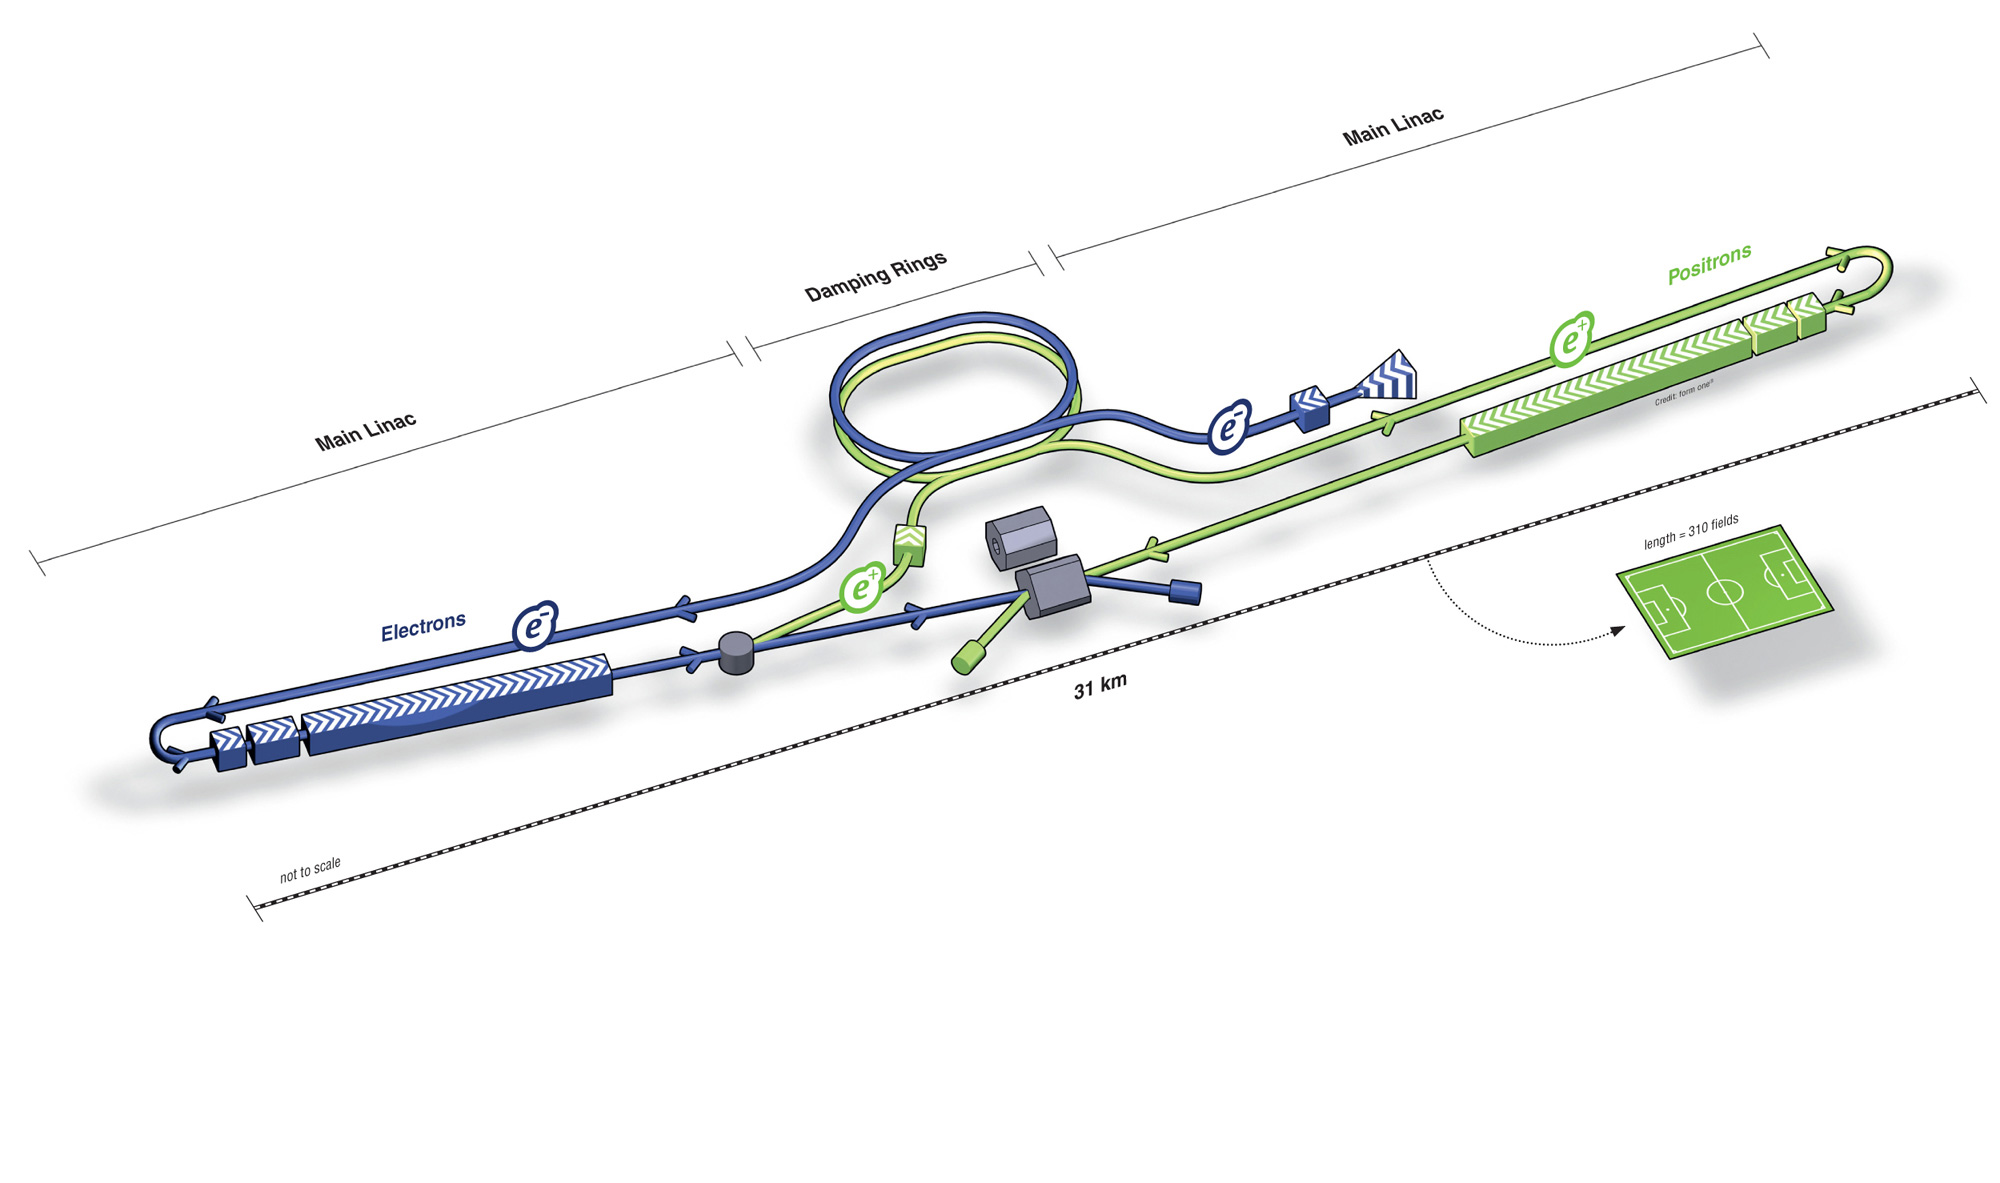
\includegraphics[width=1\textwidth,natwidth=2000,natheight=1183]{ILC_Diagram.jpg}
\caption{ILC Concept Schematic \cite{ILC:Images}}
\end{figure}

\subsubsection{Goals \cite{ILC:TechnicalDesignReport}}

\begin{enumerate}
  \item Measure the mass, spin, and interaction strengths of the Higgs boson.
  \item If discovered, measure the number, size, and shape of any TeV-­‐scale extra     dimensions.                                         
  \item Investigate the lightest supersymmetric particles, possible candidates for dark matter.
\end{enumerate}

\subsubsection{Spin-offs}

There are two types of spin-offs. The first is a reappropriation of innovative
technology originally developed for scientific research. A remarkable case in particle
accelerators research, for example, is the spilling over of high performance
electromagnetic steel specifically improved and fabricated as the iron core for accelerator magnets. The electric machinery industry has combined the high performance electromagnetic steel with substantive progress in electromagnetic field analysis software to manufacture a variety of electric machinery with lower and lower power loss rates. 

Another example is a spilling over of newly developed systems/subsystems themselves and/or common technology thereof to related industry sectors. A conspicuous illustration of this case is seen in the expanding applications of the electron linac, which was initially developed solely for nuclear and high energy physics research, to the medical and non-destructive inspection industries. Another well-known example is the growing application of superconducting magnets, having been greatly improved as an outcome of its successive adoption in particle accelerators, not only to industrial sectors such as medical therapy, material research, and power generation/transmission, but also to a magnetic levitation, ultra-high speed public transportation system. \cite{ILC:SpinOffReport}
 
\subsubsection{Feasibility}

%todo not a lot of analysis here, just facts and figures
The 500 GeV ILC technical design presented in the ILC Technical Design Report (TDR) has been developed based on an extensive R\&D program. The R\&D has
successfully demonstrated the goal of 35 MV/m accelerating gradients in test stands and 31.5 MV/m in installed cryomodules with beam loading, using niobium cavities with no more than two surface-preparation processing cycles. Cavity fabrication to these specifications has been industrialised, with qualified vendors in Europe, North America, and Asia. 

With this accelerating gradient, the total length of the 500 GeV ILC is 31 km. The effects of the electron cloud in the positron damping ring have been studied experimentally, leading to the proven techniques included in the TDR design for its mitigation. The fast kickers needed to inject and eject beams from the damping rings have been developed. The ability to achieve the small final focus spot size is being demonstrated in a test facility and gives confidence that the goal of several nm vertical spot sizes will be achieved. 

The final focus and interaction region, including the detector push-pull system needed to allow two detectors to take data sequentially, has been designed. The TDR design and the R\&D results have been judged sufficient to begin the detailed, site specific design and construction stage once international negotiations for starting the project have been concluded. Remaining work includes beam tests in multi-cryomodule facilities now under construction to assess such topics as beam stability, low level RF controls and field emission behaviour; as well as further industrialisation of SCRF cavity and cryomodule components, value engineering, and detailed site-specific engineering design. \cite{ILC:OtherReport}
 
\subsubsection{Cost \& Location}


Global Design Effort produced a “value estimate” of \$7.8 billion with 23 million person hours ($\sim$13,000 person years) of additional labour.
The host country for the accelerator has not yet been chosen and proposed locations are Japan, Europe (CERN), and the USA (Fermilab). Japan is considered the most likely candidate, as the Japanese government is willing to contribute half of the costs, according to the coordinator of study for detectors at the ILC .
 
\subsubsection{Time scale}

\begin{tabular}{p{2cm} p{12.5cm}}

2004: & Decision to use super conducting technology \\
2005 & Global Design Effort completes a baseline design for the ILC. \\
2007 & A more detailed Reference Design Report (RDR) published in 2007, which provides a technical description of the project and includes an initial value estimate. \\
2013: & The Technical Design Phase (TDP) produced technical design of the project in order to demonstrate its feasibility to all involved governments so the ILC can be approved and eventually built - the final version of the TDR was delivered to the International Committee for Future Accelerators (ICFA) on June 23rd 2013. \\
2015: & The host country is expected to be finalised around 2015 at a meeting of leaders from participating countries. \\
2015-2026: & Construction of ILC estimated to take 20 years \\

\end{tabular}

     \end{subsection}
     \begin{subsection}{CLIC}
         Compact Linear Collider (CLIC) is an anticipated high energy and high luminosity Positron-Electron linear accelerator. Positrons and electrons are fundamental particles that annihilate to produce a burst of energy known with great accuracy, making a cleaner collision. This makes it easier to pick out relevant data from background information.

The intense energy appears in the formation of numerous new particles thus opening a doorway to novel physics. CLIC would be used to compliment the Large Hadron Collider (LHC) by probing areas of interest highlighted by LHC research with a higher degree of precision than is provided by proton- proton collisions. According to CERN, CLIC will not only offer the opportunity of precise measurements of mass and couplings of new particles discovered at the LHC, but will also extend the discovery reach for particles that suffer from low production cross-section at the LHC. \cite{LHC:CP:Higgs}

\subsubsection{Design}

The LHC is based on a circular accelerator; however, when high-energy electrons and positrons are forced on a curved track they emit Synchrotron (electromagnetic) radiation, losing energy. To overcome this restriction and reach higher energies, electrons and positrons must accelerate along a straight line. As a linear collider, CLIC will use two linear accelerators, ‘two-beam acceleration’ scheme, drive and main beam; One beam for electrons, whilst the other beam is for positrons. The two accelerators will point directly at each other, synchronously shooting beams of particles that collide head on at the centre of a detector.

At the collision point, where bursts of particles are produced in the electron–positron interactions, there will be a detector. The detector is filled with consecutive detection layers. The particles cross the different detector layers in which signals generated by their passage produces a collection of thorough knowledge about each particle, such as its energy, electric charge and type.

CLIC is designed to have two detectors where only one is to be used at a time. This means that the detectors will lie on a large ‘push–pull’ platform that is moved across the collision point. With two detectors, one will be able to verify the results of the other, which will be imperative for confirming new findings.

\subsubsection{Physics Potential}
 
The Higgs physics potential at CLIC would be extraordinary, due to the large energy range of CLIC. Since being discovered at the LHC, the Higgs Boson requires a more precise study at different stages of energy production and decay modes. At CLIC, this would require approximately 125 GeV of energy. At an energy range of <500GeV at CLIC, the Z recoil from HZ production could be measured, offering mass determination (only measured using lepton colliders) and model-independent coupling. At a higher energy ($\sim$1 TeV) at CLIC, the top Yukawa coupling and tri-linear Higgs self-coupling could be measured using double Higgs production.
At the highest energy at CLIC of $\sim$ 3 TeV, the branching fraction of rare processes (e.g. decay into Muons) would be determined.
 
There is a top Quark Physics potential at CLIC, where there may be the possibility of a hint to the physics Beyond Standard Model (BSM). This is because the heaviest Standard Model Particle couples most strongly to Higgs Field, which CLIC has the energy range to investigate. The top quark mass can be precisely be determined and a direct reconstruction of top quarks from decay products at energies above the production threshold will be produced.
 
At the LHC, decay chains of strongly interacting supersymmetric particles can abundantly produce heavy Sleptons, Charginos and Neutralinos however sometimes these chains are not able to access all states. Instead, CLIC can thoroughly look for new particles with electroweak charges through exploring the TeV region. \cite{CLIC:Concept}

The precise mass and coupling measurements that can be performed at CLIC allow us to address fundamental questions integral to the mechanism of Supersymmetry, aspects of unification, and the feasibility of the lightest Supersymmetric particle as a dark matter thermal relic.” \cite{CLIC:Concept}
 
\subsubsection{Feasibility}

The CLIC Test Facility (CTF3), CERN has already started testing the feasibility of requisite technologies: power extraction, two-beam acceleration and recombination, and beam stabilisation. \cite{CLIC:DriveBeam}

CLIC requires an accelerating gradient of 100MV/m; however, superconducting accelerating cavities have an accelerating gradient restriction of approximately 60MV/ (where above this limit the superconducting properties are lost). Therefore CLIC will require a room temperature, less power-efficient accelerating cavity, where for the same collision energy it allows a shorter accelerator length. Where for CERN the total average power consumption was 200MW during peak consumption whilst LHC was in operation, CLIC power consumption is estimated to be 415 MW, at 3 TeV, which is more than double that for CERN. \cite{CERN:Powering}

During tests, the insides of the room temperature copper cavities become damaged; this needs to be resolved (although plating with tungsten or molybdenum may be a solution). Another obstacle to CLIC, would be to narrow the beams to a nanometer at the collision point. [4] Stability and accuracy is of utmost importance, as minute errors in parameters such as phase at source and beam charge will have a collective effect on the luminosity of the beam. \cite{CLIC:DriveBeam}

At the same time, new particle detectors will need to be designed to be able to cope with the physics at 3 TeV of centre-of-mass-energies and be able to operate efficiently in the CLIC machine environment. \cite{CLIC:Concept}

A major challenge for CLIC will be the manufacture of huge numbers of high strength focusing quadrupole magnets for the drive beam. Manufacturing rates of about 50 magnets per day will be required, and this is way beyond present capabilities. \cite{CLIC:STFC}
 
\subsubsection{Time scale}

\begin{tabular}{p{2cm} p{12cm}}

2012: & Finalise the CLIC Conceptual Design Reports, establish feasibility \\
2012-2016: & Project development phase, producing a project implementation plan for a CLIC construction project by 2016 \\
2016-2017: & Decision about the next project at the energy frontier \\
2017-2022: & Project implementation Phase, including an initial Project Preparation Phase to lay the groundwork for full construction \\
2022-2023: & CLIC construction set-up \\
2023-2030: & Construction of CLIC energy stage, making use of a significant fraction of the hardware developed during the Project Implementation Phase. \\
From 2030: & Commissioning of CLIC \\

\end{tabular}



     \end{subsection}
     \begin{subsection}{TLEP}
         \subsubsection{Goals}

TLEP, Triple Large Electron Positron, is an $e^+ e^-$ circular collider of circumference 80km. It will probe the properties of the Higgs H(126) boson with unmatched accuracy thanks to greater luminosity compared to other designs \cite{TLEP:Review}. In an effort to complete the Standard Model of particle physics, TLEP will also investigate the properties of the Z and W bosons and the top quark. 

Mapping the electroweak symmetry-breaking parameters will lead to stringent Standard Model closure tests. TLEP expects to be able to take direct measurements of the mass of W and top quark with an order of magnitude improvement and improve on the mass of Z pole by two orders of magnitude. \cite{TLEP:Janot}

\subsubsection{Technical Specification}

\begin{figure}[!htb]
  \centering
  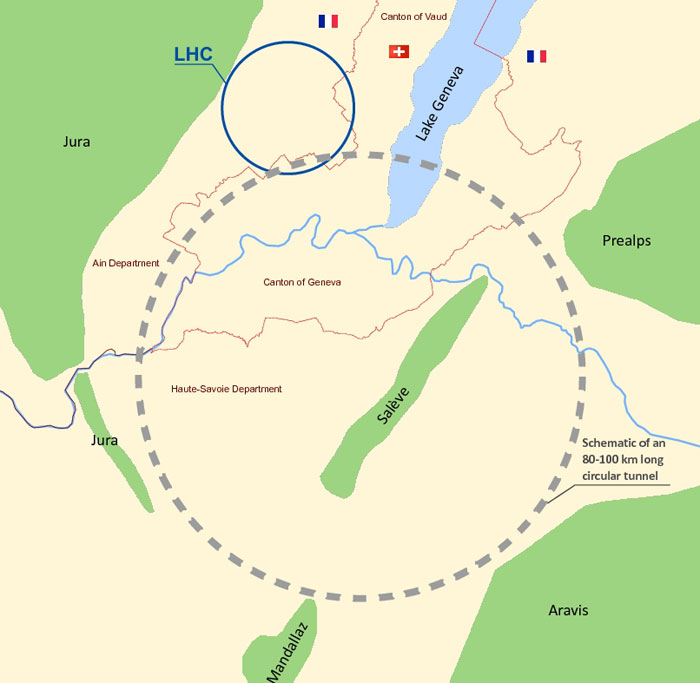
\includegraphics[width=0.6\textwidth,natwidth=700,natheight=683]{TLEP_Diagram.jpg}
  \caption{Proposed TLEP site next to LHC}
\end{figure}

TLEP's primary potential site is an 80km ring at CERN encompassing the LHC along part of the circumference. The design began as LEP3, a proposed improvement to the LHC which has been put aside in favour of TLEP due to its superior parameters, the fact it can be implemented without halting the operation of the LHC and the upgrade potential \cite{TLEP:Luminosity}. Table \ref{TLEP:Specs} shows a summary of the luminosities achievable with TLEP alongside LEP3 design for comparison. Luminosity figures for TLEP are upwards of one order of magnitude greater than any other proposed design.

\begin{table}
\centering
\begin{tabular}{l|cc}
  & LEP3 & TLEP \\
  \hline
  Circumference & 26.7km & 80km \\
  Max. Beam Energy (GeV) & 120 & 175 \\
  Luminosity @ 350 GeV ($cm^{-2} s^{-1}$) & \textendash & $0.7 \times 10^{34}$ \\
  Luminosity @ 240 GeV ($cm^{-2} s^{-1}$) & $10^{34}$ & $5 \times 10^{34}$ \\
  Luminosity @ 160 GeV ($cm^{-2} s^{-1}$) & $ 5 \times 10^{34}$ & $2 \times 10^{35}$ \\
  Luminosity @ 90 GeV  ($cm^{-2} s^{-1}$) & $2 \times 10^{35}$ & $10^{36}$ \\
\end{tabular}
  \caption{Parameters for performance of LEP3 and TLEP \cite{TLEP:AccNews}}
  \label{TLEP:Specs}
\end{table}

The main operational mode of TLEP will be at 240 GeV in order to function as a Higgs factory, however TLEP will be operating between 90 GeV, to probe the Z pole interactions, through 160 GeV to investigate W bosons, up to 350 GeV to investigate the properties of the top and anti-top quarks ($t\bar{t}$). The substantially higher luminosity compared to other designs comes from the 4 interaction points possible with the circular design, resulting in a greater number of observable interaction events per year. These specifications will result in the observation of roughly 2 million Higgs decays over a five year exposure \cite{TLEP:CERNReport}. Unparalleled beam energy accuracy is achieved by the method of transverse polarisations of the beams \cite{TLEP:Review}.

\subsubsection{Technical Feasibility}

The main focus of R\&D and cost driver will be the power requirements of the RF system. Currently CERN has a contract with France's main energy supplier EDF for 200 MW \cite{TLEP:Luminosity}. Early estimates on the power requirements of TLEP running at 175 GeV beam energy will be in the region of 280 MW, using scaled \textendash up values from the LHC and other projects. Synchrotron radiation is the main source of power loss dnd this is the main area for R\&D. The current design study benchmark is 54-59\% efficiency of the RF system \cite{TLEP:Review}. At present the extraction of 100 MW of power in the form of heated water is a design consideration that has yet to be addressed.

The interference of beam-beam interactions resulting in loss of power of the beam and in turn lower luminosity is known as beamstrahlung and must be mitigated in a successful circular collider even though the effect is far less than for linear models \cite{TLEP:Luminosity}. Estimates of acceptable momentum are in the region of 2-2.5\%. Simulations show that with a momentum acceptance of 2.5\% a beam lifetime of 460$\pm$50 s is achievable \cite{TLEP:EnergyRestriction}. Another option is to increase the ratio of horizontal to vertical emittance – producing flattened beams. LEP showed that an emittance ratio of 250 is achievable, however R\&D is needed to bring this figure closer to that of modern light sources of O(2000).

For an upper limit of the beam lifetime due to Bhabha scattering of O(1000s) 1\% of the total beam energy needs to be reintroduced every 10s \cite{TLEP:Janot} \cite{TLEP:CERNOverview}. This requires an injector and separate accelerator ring working alongside the primary ring that must be designed and considered for injector strength, power consumption and the shielding required to block the accelerator ring from the detectors. 

Detector systems are yet to be designed but those of the LHC, PEP II and KEKB experiments, among others, can be used as benchmarks. The unprecedented quantity of data available from such high luminosities requires evaluation of computing needs against currently used systems. 

\subsubsection{Cost and Schedule}

It is expected that the initial design study, reporting fully on the above main technical points, will be completed by 2015. This will be followed by an in depth conceptual and R\&D study phase with technical design of critical components to be completed by 2017-18 \cite{TLEP:CERNOverview}. These findings can then be presented at the next European Strategy update after which an informed decision on the next high-energy frontier project can be carried out and properly implemented. Construction could begin by 2020 with completion and operation by 2030. 

TLEP's preliminary cost estimates have been based largely on the fact that the design utilises fairly mature technologies and many of the contributions to cost estimates have been arrived at by scaling up existing projects. However with the technical challenges still to overcome it is impossible to arrive at anything but very rough estimates of an overall budget. Current estimates place the total cost at 7 billion Swiss Francs, of the same order as the LHC and ILC design \cite{TLEP:Janot}. Of this value half is projected to be the digging of the tunnel itself and it is important to note detector cost has not been factored into this value.

\subsubsection{Potential}

TLEP has a highly promising potential upgrade path. Following the fulfilment of the experimental objectives within a reasonable lifespan of the project ($\sim$40 years from present), TLEP can undergo combination with the LHC to form the VHE-LHC, a 100 TeV proton-proton collider with the LHC serving as an injector ring \cite{TLEP:Janot}. This provides a robust long-term vision for high energy physics and the CERN facilities with the promise of precision measurements and potential for discovery at an energy frontier higher than any alternative. The return of investment on each facility by repurposing them together financially trumps the costs of all other long-term design schemes as they stand at present.

     \end{subsection}
     \begin{subsection}{LHeC}
         \subsubsection{Overview \cite{LHeC:Birmingham}}

The LHeC has been proposed as a colliding beam facility at CERN. It will exploit the high energies already available at the LHC for lepton-nucleon collisions. An existing LHC proton or heavy ion beam will be used to collide with a new, high energy, electron beam; this will occur simultaneously with the LHC’s current proton-proton experiments.
 
In the current design (figure 1), the electron beam is accelerated passing multiple times through a pair of linear accelerators in a racetrack configuration, producing an energy of 60 GeV at the interaction point. This results in an unprecedented kinematic range for lepton-nucleon scattering: the centre of mass energy will be 1.3 TeV The luminosity of $10^{33}$ \textemdash $10^{34} cm^{-2}s^{-1}$ is two orders of magnitude larger than previous similar proposals.

\begin{figure}[!htb]
\centering
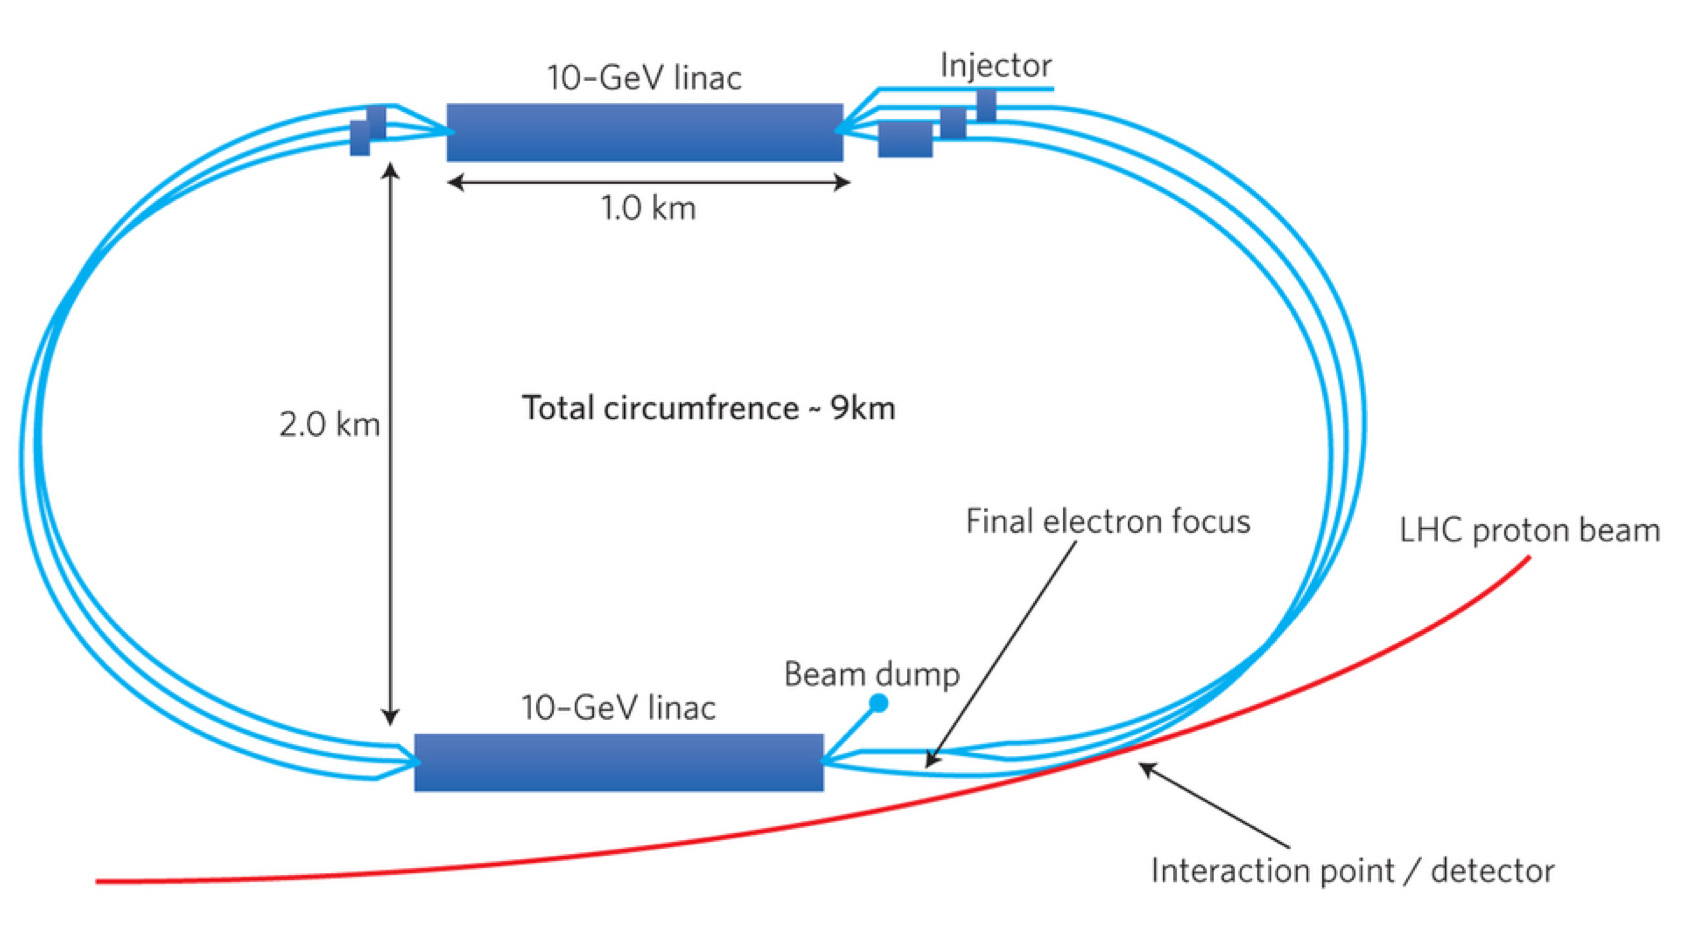
\includegraphics[width=0.9\textwidth]{LHeC_Diagram.jpg}
\caption{The current layout of the proposed electron ring (blue) next the a section of the LHC’s proton accelerating ring (red).
}
\end{figure}

\subsubsection{Goals}

The goals of the LHeC are as follows:
\begin{itemize}
\item Explore quantum chromo dynamics in greater detail with greater precision.
\item Examine the strong nuclear interaction in greater detail with greater precision.
\item Potentially use it as a rich source of the Higgs Boson and thus explore its interaction strength, mass and spin.
\item Able to produce Charm, Top and Bottom quarks for greater examination.
\end{itemize}
As the collider will use electron-proton collisions it will make it an invaluable tool in the examination of the structure of the proton, as it will provide cleaner reactions than are currently possible at the LHC.
 
\subsubsection{Feasibility}

The proton side of the design will incorporate the already functional proton accelerator that is built at the LHC and thus there will be no feasibility issues with this. On top of this the current LHC experiments can continue to run during the construction of the collider and will continue to be run once it is operational, there is a small risk of interruption during the tunnel excavation phase due to the proximity to the LHC ring. This then means that the LHC will continue to push the energy boundaries whilst the LHeC can examine the structure of the proton and the Higgs boson in greater detail. Also if any new discoveries are made in the energy scale of 1.3TeV at the LHC it will be possible to test them with greater precision using the LHeC.
 
The electron beam will not use any new technologies in its creation; the only issue that will arise is attempting to match its circumference to that of the proton ring. Though civil engineers have already considered this and have declared it feasible. \cite{LHeC:Report}
 
Overall the design is feasible, and this will not be a problem is implementing the construction of the LHeC.
 
\subsubsection{Spin Offs}

There are few unique spin offs relevant to this collider, as its goal is to probe the structure of the proton with more precision it is entirely possible that spin offs will emerge after its construction that may result from this greater understanding.
 
The main, somewhat generic, spin off is the improvement of data transfer in computing. This will allow communication to occur at much greater rates between computers and allow much larger arrays of data to be generated faster.
 
A more unique spin off is the improvement of viability of PET due to SCRFs. Superconducting Radiofrequency acceleration is the production of high quality and energy X-Rays using Inverse Compton Scattering (ICS). ICS is the transfer of energy from an electron to a photon. ICS only exists in nature at the accretion disk of a black hole, where slow photons are collided with fast electrons causing X-Ray spectra. However it may be possible to generate these frequencies colliding a fast proton and electron at LHeC.
 
\subsubsection{Cost}

Detailed cost analyses have yet to be produced, as the project has not gained much momentum in the physics community. One estimate put the cost at $\sim$\$50M \cite{LHeC:Zimmermann}. This costing seems very low and may fail to take into account any of the cost considerations involved in digging the tunnels. Though because a large part of the design incorporates the already functional LHC the costs would be lower than other proposed colliders.
 
 
\subsubsection{Time scale}

As all of the technology required is already in production and used in modern colliders there would be very little (possibly no) research and development time needed before construction could begin.
 
The total estimated time; from starting the assembly of the main detector elements on the surface to the commissioning of the detector underground is 30 months. The field map would take one extra month.
 
\subsubsection{Conclusion}

Though the design is feasible, the costs potentially low and the time scale short; construction of this collider is not recommended. This is because the physics that this collider could explore is not nearly as interesting as that proposed by other colliders. The structure of the proton may be further explored in higher energy experiments at CERN’s LHC and the commission of a new facility to explore this is unnecessary. Finally other proposed colliders provide a much cleaner and precise process to look at the mass, interaction strength and spin of the Higgs particle.
     \end{subsection}
     \begin{subsection}{Muon-Muon}
         \cite{Muon:WhitePaper}
\cite{Muon:Geer}
\cite{Muon:Collide}
\cite{Muon:Nature}
\cite{Muon:CERNCourier}
\cite{Muon:ProtonBeam}
\cite{Muon:Feasibility}
\cite{Muon:MICE}
\cite{Muon:PDG}

\subsubsection{Muons}

Muons ($\mu^-$) are elementary particles, and like electrons, are classified as leptons with spin $-\frac{1}{2}$ and charge of $-1$. However, muons have a mass of mμ = 105.7 $MeV/c^2$, which is about 200 times the mass of the electron (me = 0.511 $MeV/c^2$). Muons are also unstable particles with a mean lifetime of about 2.2$\mu s$. Its dominant decay process is given by:

\begin{equation}
    \mu^- \rightarrow e^- + \bar{\nu_e} + \nu_{\mu}
\end{equation}

where it decays into an electron, an anti-electron neutrino and a muon neutrino. The muon’s antiparticle, the anti-muon ($\mu^+$) decays into similar products: 

\begin{equation}
    \mu^+ \rightarrow e^+ + \nu_e + \bar{\nu_{\mu}}
\end{equation}    
 
where the products are simply the charge conjugates of the muon’s decay products.
 
\subsubsection{Muon Acceleration Program (MAP) and Muon Colliders}

With the recent interest in a lepton collider to be built as the next-generation collider after the LHC in CERN, there have been efforts within the scientific community to push forward the idea of a muon collider, compared to an electron-positron ($e^+ e^-$) collider such as the ILC or CLIC.
 
The United States Muon Accelerator Program (MAP) was set up in 2010 as a joint organisation between the Neutrino Factory and Muon Collider Collaboration (NFMCC) and the Muon Collider Task Force (MCTF) under the direction of the U.S. Department of Energy. Its goal is to develop the concepts and technologies required for the construction of Muon Colliders and Neutrino Factories for the physics community, which would hopefully further push the energy and technology frontier in particle physics research.
 
Muon colliders provide an interesting and attractive alternative when it comes to lepton colliders, especially in terms of the collider’s physics reach and potential development cost. This is mainly due to the muon’s aforementioned properties which allow higher efficiency while being able to achieve a higher-energy collider. Muon colliders are also a potentially unparalleled Neutrino Factory, capable of allowing physicists probe into Beyond Standard Model Physics in a world-class neutrino research facility. However, the concept of a muon collider is mainly plagued by its technical feasibility, as current goals of a muon collider would require more years of research and development into innovative, new technology that currently have not necessarily been shown to be demonstrable at a laboratory scale.
 
\subsubsection{Physics Reach/Goals}
 
The current proposal put forth for a muon collider would be a circular multi-TeV collider that could reach centre-of-mass energies of 4 TeV, with a luminosity goal of $10^{34}$ \textemdash $10^{35} cm^{-2} s^{-1}$. The diameter of such a collider would be approximately 2-3 km, which would fit easily within the footprint of the Fermilab site. The Muon Collider’s early stages would also see it serve as a Neutrino Factory, which would provide the physics community with a world-class neutrino research program.
 
The current concept to such a monumental project would be a staged approach to the construction, where at each stage, the facility will have a unique and important physics reach with increasing complexity; this begins with a Neutrino Factory facility (nuSTORM, nuMAX and nuMAX+, with increasing intensity), followed by a Higgs Factory capable of producing up to 13,500 high resolution Higgs events a year, and culminating in a multi-TeV muon collider.
 
\subsubsection{Neutrino Physics}
 
Muon colliders provide a promising source of neutrinos needed to produce an intense neutrino beam for research. Previous laboratory sources of neutrinos only produce one dominant flavour of neutrinos. Charged kaons and pions were allowed to decay in long, straight decay channels into muon neutrinos, with a small percentage of three-body decays that produce electron neutrinos. This small percentage of electron neutrinos was considered to be an undesirable contamination in the otherwise “pure” neutrino beam. Due to the muon’s dominant decay into two different flavours of neutrinos, it is certain that the decay produces 50\% of each flavour, eliminating the contamination problem. Hence, they represent a new and better way of producing an intense neutrino beam required for high quality neutrino research.
 
\begin{figure}[!htb]
\centering
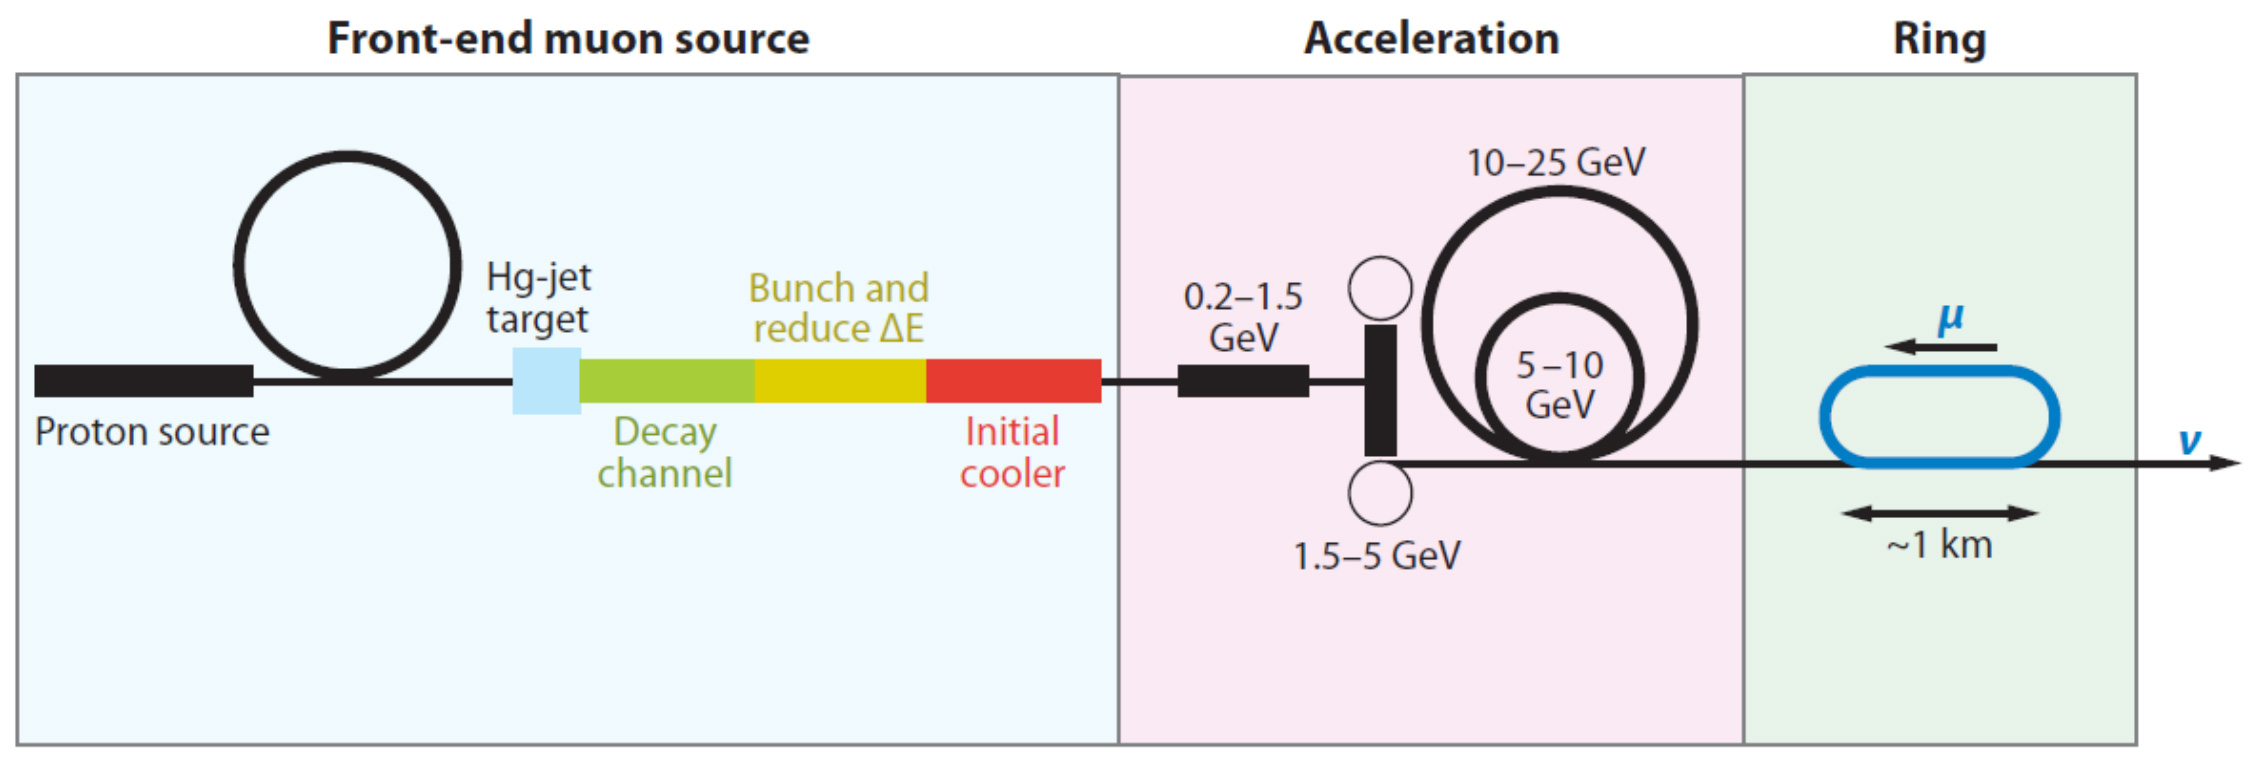
\includegraphics[width=1\textwidth]{Muon_Neutrino.jpg}
\caption{Schematic Diagram of the Neutrino Factory Planned for a Muon Collider}
\end{figure}
 
Protons are fired at a dense mercury (Hg) target, where the resulting collision produces $\pi \pm$ that are allowed to decay and into daughter muons. These daughter muons then undergo phase rotation before being cooled for acceleration into a muon storage ring.
 
\subsubsection{Multi-TeV Collider}
 
When working with charged particle in colliders, the main efficiency concern would be energy loss through synchrotron radiation. When a charged particle is accelerated around a curved path, it emits synchrotron radiation, given by:

\begin{equation}
    P = \frac{
        e^2 c \gamma^4
    }{
        6 \pi \epsilon_0 \rho^2
    } = \frac{
        e^2 E^2 B^2
    }{
        6 \pi \epsilon_0 m^4 c^5
    }
\end{equation}
 
where $P$ is the power radiated, $e$ is the electron charge, $c$ is the speed of light in vacuum, $\gamma$ is the Lorentz factor, $\rho$ is the radius of curvature of particle track, $E$ is the electron energy, $B$ is the magnetic field and $m$ is the mass of the particle. The key is that the power radiated scales as $m^{-4}$. The biggest difference between a muon and an electron is their masses; therefore, this relation is particularly important when comparing the differences between an electron and a muon collider.
 
Compared to a linear $e^+ e^-$ collider, a muon collider would instead be a circular collider, much like the LHC. This is because unlike electrons, muons suffer much less synchrotron radiation due to its larger mass. Since the ratio of masses $\frac{m_{\mu}}{m_e}$ is about 200, $\frac{m_{\mu}}{m_e}^4 = 2 \times 10^9$ would mean that these radiation effects will be greatly reduced. Hence, a muon collider would enjoy all the benefits that come from circular colliders, such as multiple circulations, multi-turn collisions and multiple interaction points that increase events observed, while also benefitting from the clean collision environment as provided from a lepton collider. These greatly increase the overall efficiency of the collider, and reduce the overall power consumption of a muon collider compared to that of a linear $e^+ e^-$ collider.
 
The ability of a muon collider to reach energy levels beyond that of even CLIC (which has a maximum energy level of $\sim$3 TeV) is also due to the large mass of the muon. The large mass of the muon, compared to the electron, means that it is also easier to accelerate muons to higher energies. Added on to the fact that muons suffer less from synchrotron radiation, means that a muon collider is able to reach energies beyond the feasibility range of a linear lepton collider, in terms of a feasible length and size.
 
\subsubsection{Higgs Factory/Measurement}
 
One of the goals that the physics community is hoping that the next collider would adequately achieve would be precise measurements of the Higgs particle, recently discovered at the LHC in 2012.  A muon collider would be a great candidate to fulfil that goal as it couples much more strongly to the Higgs field (and hence the boson) due to its larger mass. In fact, as the mass-dependent Higgs coupling is proportional to the mass of the lepton, the coupling of the Higgs to a muon is approximately $\frac{m}{m_e}^2 = 4 \times 10^4$ times larger than that of an electron’s.
 
As the muon collider would be a circular collider, this also allows multiple interaction points which increase the event rate and allow multiple simultaneous experiments. The reduction in beamstrahlung effects, which refer to a type of synchrotron radiation emitted from beam-beam interactions at the interaction point due to electromagnetic field interactions of charged particles, also mean that a muon collider can have more precise beam-energy constraints and a sharper distribution for signals that allow for greater precision in mass and width measurements.

\subsubsection{Technical Feasibility}
 
The main challenge of muon colliders lies in the fact that compared to other more robust and proposals such as the ILC, it would require much more advanced technology that are not necessarily demonstrable in a laboratory setting as of now. To achieve the ultimate goal of a multi-TeV collider, it would require a powerful proton linac and target station, the ability to cool muons down to a narrow, cold beam, and finally a suitable acceleration scheme for rapid beam acceleration.
 
To achieve the high-power proton linac required for muon production, the Mercury Intense Target (MERIT) Experiment was set up to develop the technology required for a target station capable of handling  more than 4MW of power. Recent results from MERIT have shown proof of a free Hg-jet target technology that is capable of handling the required proton beam power without dispersion of jet target due to shock and/or vaporisation, and without damping due to the strong magnetic field from the capture solenoid ($\sim$20T).
 
However, the biggest technological challenge lies in muon cooling and acceleration. As the muons are produced from decay processes after smashing protons into a dense Hg target, the energy spread of muons is significantly large. The challenge is to be able to cool these muons down to a size small enough so that they form an extremely narrow cold beam suitable for acceleration. Moreover, given the short lifetime of the muon, a rapid acceleration system is required to accelerate these cooled muons before they decay.
 
To tackle these issues, the International Muon Ionisation Cooling Experiment (MICE) was set up to develop novel and innovative technologies in ionisation cooling in order to achieve the 6-orders-of-magnitude cooling channel required.
 
\begin{figure}[!htb]
\centering
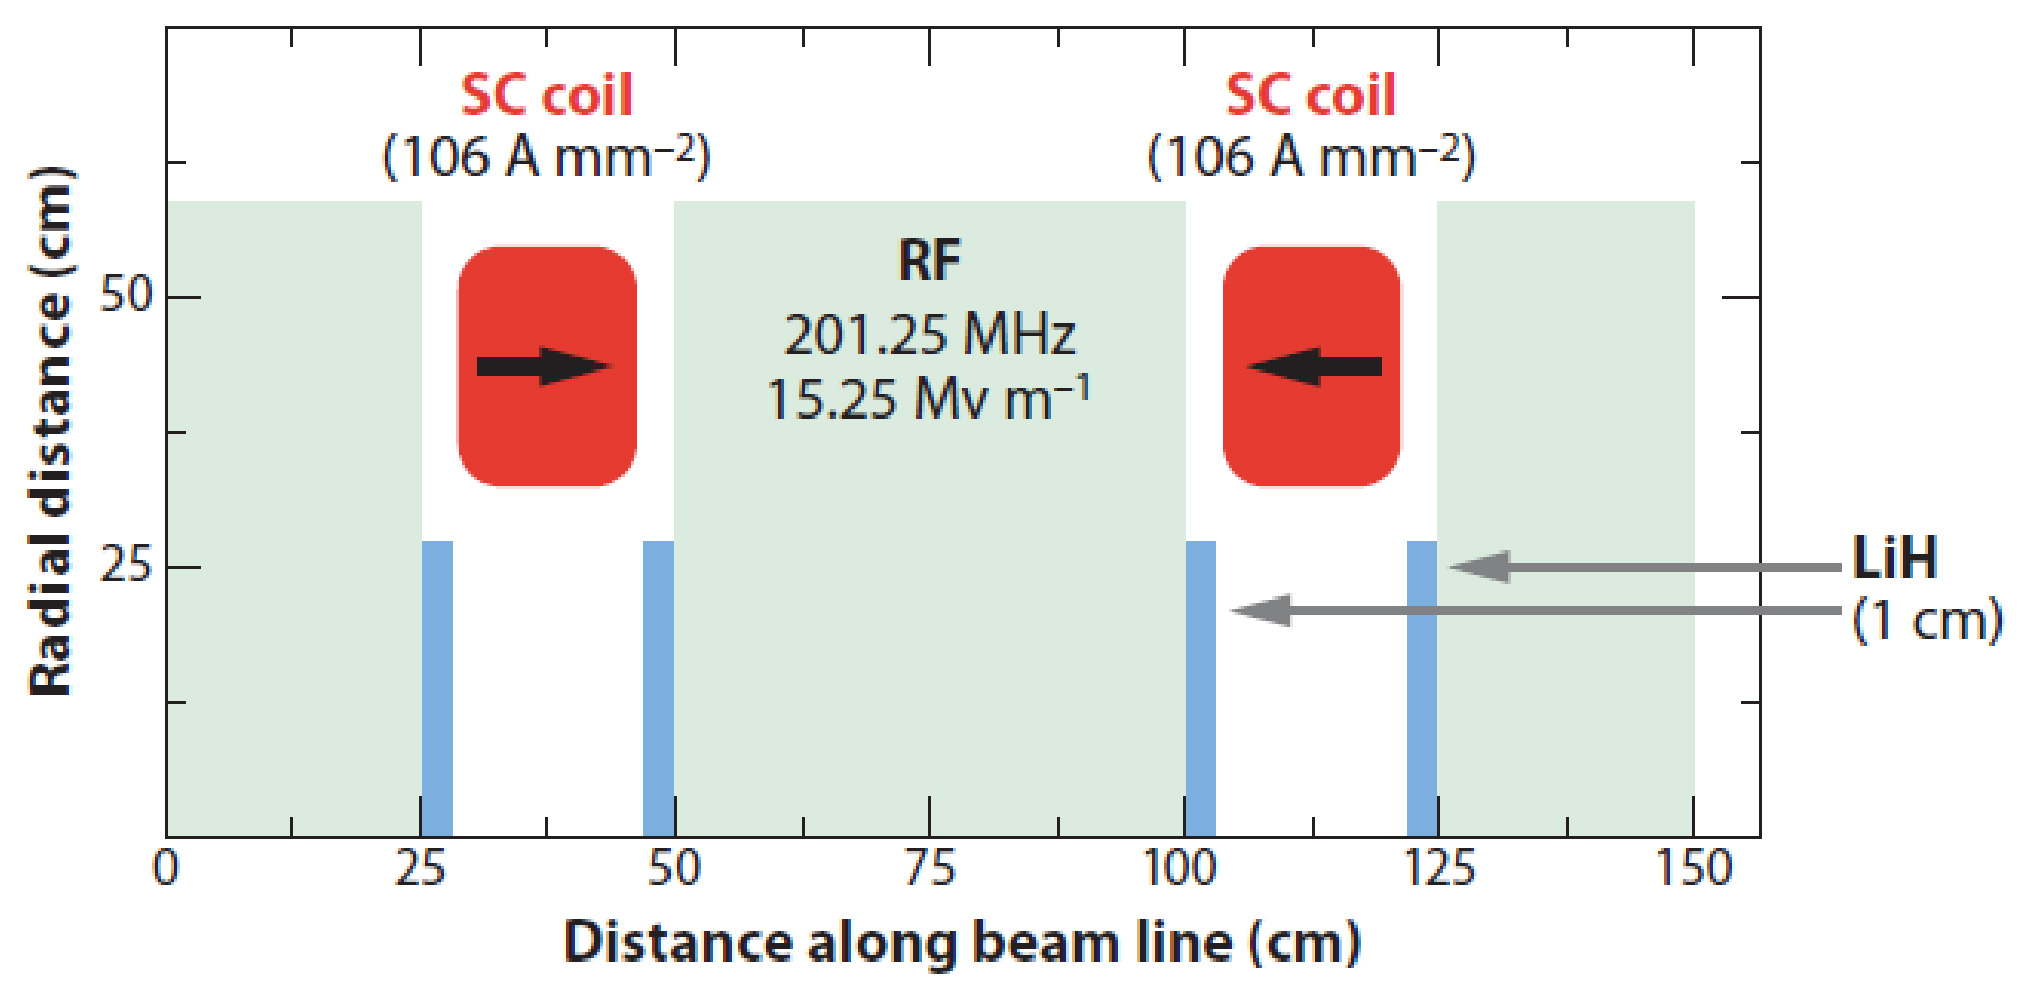
\includegraphics[width=0.7\textwidth]{Muon_Cooling.jpg}
\caption{Schematic Diagram of the Ionisation Cooling Process}
\end{figure}
 
The rate at which normalised transverse emittance $\epsilon$ is lost as muons of energy $E$ travel through a material with radiation length $L_R$ is given by:
 
\begin{equation}
    \frac{d \epsilon}{ds} = - \frac{dE}{ds} \frac{\epsilon}{E} + \frac{\beta_{\perp} (0.014)^2}{2 E m_{\mu} L_R}
\end{equation}
 
where $\beta_{\perp}$ is the betatron function (which represents the focusing strength at the absorber), $m$ is the mass of the muon and $\frac{dE}{ds}$ is the energy loss through ionisation loss. In order to reduce their longitudinal and transverse momenta, the muons are passed through a series of absorbers of low Z (with large $L_R$) such as lithium hydride and to use strong solenoids to focus the beam (to reduce $\beta_{\perp}$). However, in order to maintain the muon’s longitudinal momentum (to form a muon beam), it goes through a series of radio-frequency (RF) cavities to re-accelerate the muons longitudinally. This reduces the overall transverse emittance of the muons.
 
According to the 2013 White Paper submitted by MAP, the first results for transverse cooling are expected from MICE by 2015 for one cooling station and no re-acceleration of muons, while the results from a full cooling cell with acceleration is expected by 2019. However, results from ionisation cooling demonstrated at a reasonable intensity of muons are expected by 2022. As observed, the technology required for muon colliders are still not demonstrable, and while great strides have been made, it is nowhere as mature or as ready as the technology needed for the ILC, or even CLIC.
 
\subsubsection{Development Cost}
 
As a muon collider still requires many years of R\&D before a robust proposal or design report can be achieved, the current development cost estimates are relatively unknown. However, given the knowledge that a muon collider would be much more compact and more efficient in terms of power consumption, it is a reasonable estimate that the cost of construction of a muon collider might be much more economical as compared to a linear $e^+ e^-$ collider. Figure \ref{Muon:Layout} shows how the muon collider would easily fit within the Fermilab site.

\begin{figure}[!htb]
\centering
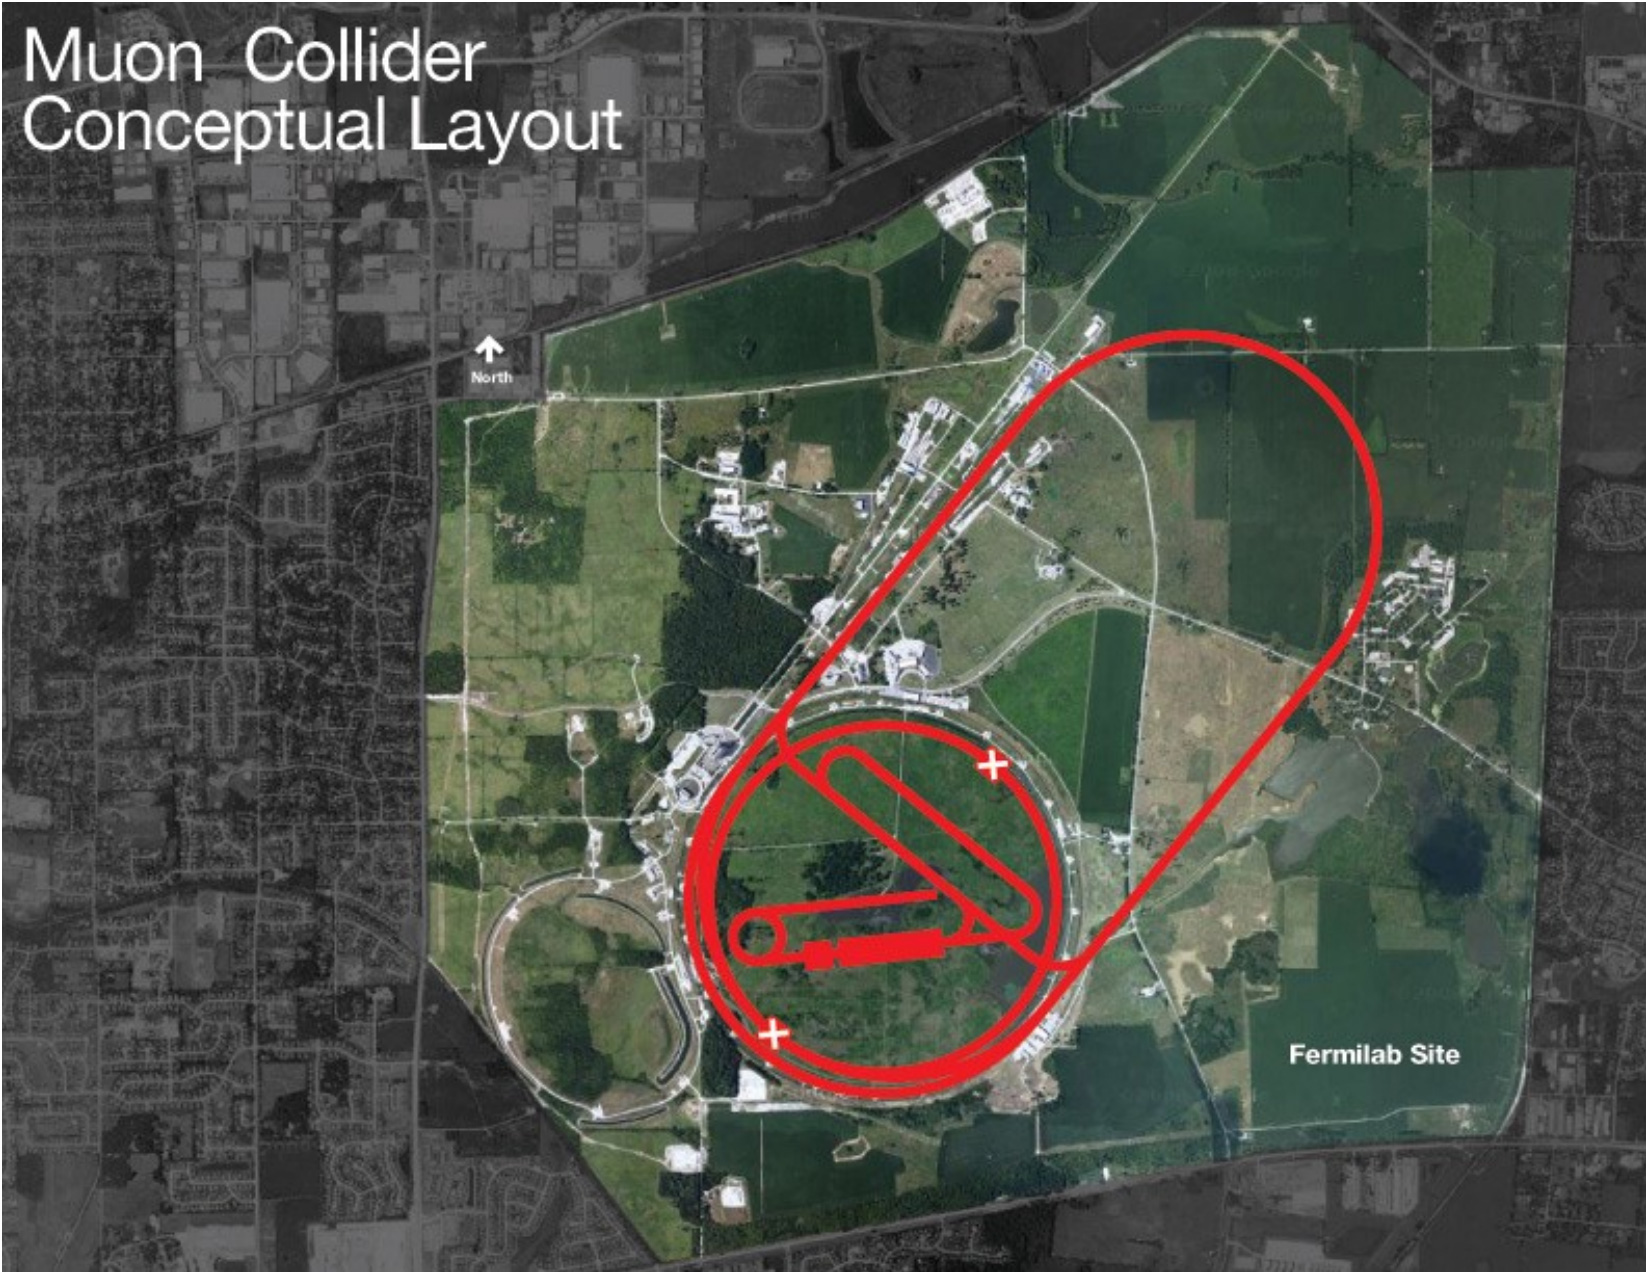
\includegraphics[width=0.6\textwidth]{Muon_Layout.jpg}
\caption{Muon Collider Layout at Fermilab}
\label{Muon:Layout}
\end{figure}
 
The staged approach to building the entire collider would hopefully reduce the required investment at each stage, further reducing the overall cost of the project. This is of paramount importance as the current site of the collider is in the United States, and given the current economic situation, the United States has been unwilling to host a large project like the ILC, let alone a relatively untested muon collider. However, given the years needed to conduct the necessary research, the economic situation of the U.S. may have drastic changes over the decades that are hard to predict.
     \end{subsection}
     \begin{subsection}{SAPPHiRE}
        \subsubsection{Introduction to $\gamma\gamma$ Colliders}
Photon colliders were originally proposed as potential extensions to linear colliders (there have been designs based on the ILC and CLIC \cite{CLIC:Multilinear}) but can also be built as independent machines. A photon collider operates using the process of inverse Compton scattering\textemdash generating  high energy gamma rays for colliding by directing a low energy laser beam ($\sim$1 eV) into a high energy electron beam (10s of GeV) i.e. the electrons transfer some of their energy to the photons \cite{Chou:Higgs}.

Gamma-gamma ($\gamma\gamma$) collisions result in a large cross section of $\gamma\gamma$ $\rightarrow$ H interactions similar to that in electron-positron colliders, e$^{+}$e$^{-}$ $\rightarrow$ ZH ($\sim$200 fb) \cite{Chou:Higgs} however the energy required for $\gamma\gamma$ collisions is a lot lower\textemdash 80 GeV electron beam energy compared to 120 GeV in the e$^{+}$e$^{-}$ colliders. This reduced energy requirement is beneficial to circular colliders as it corresponds to a decrease in the synchrotron radiation power by a factor of 5 and makes the option of building a circular photon collider at Fermilab named HFiTT\textemdash Higgs Factory in Tevatron Tunnel\textemdash a possibility \cite{Chou:Higgs}. 

The lower energy required for Higgs production makes photon colliders a good option for a new low energy, cost effective Higgs factory. Additional advantages of photon colliders include: no positron source is required, no damping rings, the high polarisation of photons and electrons and the ability to reuse existing infrastructure or extending ones that would be built anyway. However the physics capability of a photon collider is not as wide-ranging as a 240 GeV e$^{+}$e$^{-}$ collider and there are design issues to overcome such as IR optics, power consumption and removal of the spent electrons \cite{Blondel:HiggsF}.
 
\subsubsection{Physics of $\gamma\gamma$-to-Higgs}
A large cross-section of 200 fb is achieved in the direct s-channel $\gamma\gamma$ $\rightarrow$ H reaction. This is an important reaction and enhancement of the signal over the background is achieved for photons of circular polarization in the J=0 state by using a polarized laser \cite{Blondel:HiggsF}.  The CP properties of the Higgs Boson can be measured directly using linearly polarized high-energy photons. In fact photon colliders are the only machines capable of measuring the CP admixture and violation of the Higgs to an accuracy of 1\% or more \cite{Chou:Higgs}.

Photon colliders can measure the H-to-$\gamma\gamma$ partial width ($\gamma\gamma$) to a precision of 1\% \cite{Chou:Higgs}, which is better than any other collider. The $\gamma\gamma$ determines the production rate of Higgs in $\gamma\gamma$ collisions and can be measured by observing the decay mode H $\rightarrow$ bb accounting for ∼57\% of total Higgs decays. In e$^{+}$e$^{-}$− collisions, $\gamma\gamma$ is measured in the H $\rightarrow$ $\gamma\gamma$ decay which has a branching fraction of 0.24\%. Therefore at the photon collider, ``the statistics for the measurement of $\Gamma$(H $\rightarrow$ $\gamma\gamma$) is higher by a factor of $\frac{\frac{0.57}{0.0024}}{4}$ $\simeq$ 60 (and will be even larger if a lower-emmittance electron source becomes available). \cite{Telnov:Photons} The H-to-$\gamma\gamma$ partial width is an important quantity in Higgs physics because the decay proceeds via an inclusive loop that could reveal heavier particles which the Higgs is unable to directly decay into\textemdash new physics potential.

\subsubsection{SAPPHiRE proposal}
SAPPHiRE (Small Accelerator for Photon-Photon Higgs Production using Recirculating Electrons) is a proposed stand-alone $\gamma\gamma$ collider that presents a cost and time efficient option for a Higgs factory capable of accurately measuring Higgs particle properties. The basic principle of operation in SAPPHiRE is based on the process of inverse compton scattering described above with the collider hitting accelerated electrons with a low energy laser beam ($\sim$3.5 eV) generating a back-scattered gamma beam for collision. By colliding photons, the limits to luminosity arising from beam-beam interactions (beamsstrahlung) of charged particles are avoided \cite{Zimmermann:SAPPHiRE}. The SAPPHiRE collider will be about 9Km in circumference and accelerate particles to 80 GeV thus making it the lowest-energy Higgs factory \cite{Bogacz:SAPPHiRE}.

\subsubsection{Technical design and parameters}                                                                                                            SAPPHIRE's design is based on a pair of $\sim$10 GeV recirculating Linacs, similar to those used for LHeC (the sapphire project emanated from the recirculating linac system at LHEC ). The collider has a Laser back scattering system able to produce a $\gamma\gamma$ peak luminosity of 0.36 × 1034 cm−2 s−1 with ECM ($\gamma\gamma$) ∼ 125 GeV. Hence it will be able to produce tens of thousands of Higgs (H) particles a year in clean experimental conditions \cite{Bogacz:SAPPHiRE}.

\begin{figure}
\centering
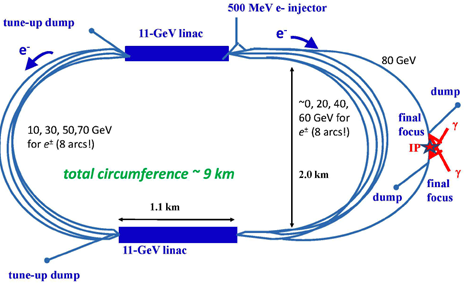
\includegraphics{sapphire1.png}
\caption{Schematic of the SAPPHiRE design based on recirculating superconducting linacs \cite{Bogacz:SAPPHiRE}.}
\end{figure}

The 80 GeV electron beam centre of mass energy required is reached by four passes through the two superconducting recirculating LINACs which increase the electron energy by $\sim$10GeV in each passing.  In comparison to the LHeC, an additional arc is required on both sides with respective beam energies of 70GeV and 80 GeV. The $\gamma\gamma$ collision point is located at the centre of the 80 GeV arc. The Compton scattering point (where gamma beams are generated) is to be located $\sim$1mm from the $\gamma\gamma$ interaction point and laser pulses are required at a frequency of 200kHz. The other laser parameters are: a wavelength of 351nm, 5J pulse energy and a long pulse duration of 5 ps \cite{Bogacz:SAPPHiRE}.

\begin{table}
\begin{center}
\begin{tabular}{l r}
\hline
\hline
Total electric power & 100 MW\\
Beam energy & 80 GeV\\
Beam polarization & 0.80\\
Beam population & $10^{10}$\\
\# of bunches per train & \textemdash\\
\# of trains per rf tube & \textemdash\\
Repetition rate & cw\\
Average bunch frequency & 200 kHz\\
Average beam current & 0.32 mA\\
RMS bunch length & 30 \textmu m\\
Crossing angle & $\geq$ 20mrad\\
Normalised horizontal emittance & 5 \textmu m\\
Nominal horizontal beta function at the IP & 0.5 \textmu m\\
Nominal vertical beta function at the IP & 5 mm\\
Nominal RMS horizontal IP spot size & 400 nm\\
Nominal RMS vertical IP spot size & 18 nm\\
Nominal RMS horizontal CP spot size & 400 nm\\
Nominal RMS vertical CP spot size & 180 nm\\
e$^{-}$e$^{-}$ geometric luminosity & $2.2 \times 10^{34} cm^{-2}s^{-1}$\\
\hline
\hline
\end{tabular}
\caption{Parameters for SAPPHiRE optimised for Higgs mass $\sim$125 GeV}
\end{center}
\end{table}

\subsubsection{Technical feasibility}
The energy loss in an arc is given by:

\begin{equation}
E_{arc}[GeV]=8.846 \times 10^{-5}\frac{(E \ [GeV])^{4}}{2\rho \ [m]}
\end{equation}

Where the bending radius, $\rho$ = 764 m (equal to the LHeC design) and the energy loss in each arc is shown in table 2. Each electron beam loses about 4 GeV in energy, which can be is compensated for by increasing the voltages of the two LINACs from 10 GV to 10.63 GV. The beams in the 70GeV arc lose the most energy due to synchrotron radiation: 1.39 GeV, or a 2\% loss \cite{Bogacz:SAPPHiRE}.

\begin{table}
\begin{center}
\begin{tabular}{c c c}
\hline
\hline
beam energy [GeV] & $\Delta E_{arc}$ [GeV] & $\Delta\sigma_{E}$ [MeV]\\
\hline
10 & 0.0006 & 0.038\\
20 & 0.009 & 0.43\\
30 & 0.05 & 1.7\\
40 & 0.15 & 5.0\\
50 & 0.36 & 10\\
60 & 0.75 & 20\\
70 & 1.39 & 35\\
80 & 1.19 & 27\\
\hline
total & 3.89 & 57 (0.071\%)\\
\hline
\hline
\end{tabular}
\caption{displays the energy losses and energy spread induced in the 8 arcs of SAPPHiRE}
\end{center}
\end{table}

The energy spread from synchrotron radiation in the arc bends is given by:
\begin{equation}
\Delta\sigma^{2}_{E}=\frac{\alpha(\hbar c)^{2}}{48\sqrt{3}}\gamma^{7}\frac{\pi}{\rho^{2}}
\end{equation}

With the geometric radius, R $\simeq$ 1 km and $\rho$ is the dipole bending radius in the arc. The total additional energy spread as a result of synchrotron radiation is only 0.071\% \cite{Bogacz:SAPPHiRE}.

The horizontal emmittance growth of the electron beam caused by synchrotron radiation poses a severe feasibility limitation and is given by:

\begin{equation}
\Delta_{\epsilon/N}=\frac{2pi}{3}\frac{c_{q}r_{e}}{\rho^{2}}\gamma^{6}\langle H \rangle
\end{equation}

Sapphire needs a smaller horizontal emmittance growth than the LHeC which has  = 13 microns at 60GeV.  Reducing the cell length and associated dipole length by a factor of 4 will reduce  at 80GeV to 1 micron, adequate for SAPPHiRE. This means the total length of the bending magnets per optical cell is reduced from $l_{bend}$ $\simeq$ 40 m in the LHeC design to $l_{bend}$ = 10 m for SAPPHiRE \cite{Bogacz:SAPPHiRE}.

Sapphire requires an emmittance ratio of $\frac{\epsilon_{x}}{\epsilon_{y}} \sim 10$, a bunch charge of 1.6 nC and an initial emmittance of $\sim$1.5 \textmu m. These parameters are achievable within the present state of the art. Hence the SAPPHiRE concept employs feasible accelerator parameters. However the main concern is whether we can get polarized beams with these parameters: a polarized low emmittance electron gun is needed. There are ongoing R \& D efforts looking into ``low-emmittance DC guns'' and ``polarized SRF guns. \cite{Zimmermann:SAPPHiRE}

\subsubsection{Advantages of Sapphire}                                                                                                              The lower beam energy of 80 GeV required to create the Higgs boson allows for efficient recirculation and a 10 times smaller Radio Frequency installation (reducing costs) \cite{Bogacz:SAPPHiRE}. For a stand-alone collider such as the Sapphire, there is no positron beam requirement and no damping rings– further large savings and simplification.

High polarization in the primary electron and the colliding $\gamma$ beams\textemdash in contrast to the case of e$^{+}$\textemdash is becoming a possibility as the Laser technology needed to generate such beams is becoming a reality. SAPPHiRE designs are cost effective (\textless \$1 billion) and take advantage of existing technology and infrastructure. The photon collider concept is applicable to ILC/CLIC as a companion capability. There is no beamstrahlung which results in a higher energy reach than electron positron colliders \cite{Zimmermann:SAPPHiRE}.

\subsubsection{Main issues}
The major design limitation of the SAPPHiRE is the unacceptable increase of horizontal emmittance in the bending arcs: The authors of SAPPHiRE solve this by reducing the dipole section length by 4 which will result in a 64 times smaller emmittance dilution however this requires 16 times stronger quadrupole magnets (quads gradient will be 16 times larger) \cite{Telnov:Photons}.

The initial normalized beam emittances quoted in the sapphire paper of 5 μm and 0.5 μm in the x and y directions respectively, correspond to best unpolarised RF gun emittances but photon colliders need polarised electrons. Currently no low emittance polarized RF guns exist (though progress is being made) \cite{Telnov:Photons:MIT}.

The high-performance laser backscattering system required in collider requires the most R \& D, though money is likely to be made from spin-offs as a result of developments in laser systems which will be beneficial in other fields of science and industry. The main problem is in achieving the lasers high repetition rate of 200kHz; it is possible to overcome this using a passive optical cavity however this is very complex. An alternative approach involves the use of a free electron laser which is cheaper and less complex \cite{Zimmermann:TLEP}.

\subsubsection{Goals and summary of possible measurements}
SAPPHiRE can measure accurately the mass, bb, WW*, and $\gamma\gamma$ decays of the Higgs boson with corresponding plausible statistical errors on these decay paths of 2\%, 5\% and 8\% respectively. In addition, the Higgs mass can be measured to a predicted accuracy of $\sim$100 MeV after 2 years of operation. Other possible decay modes that should be observable include h $\rightarrow$ ZZ* and H $\rightarrow$ Z$\gamma$ but no studies have been made yet. Also, there is the possibility of observing H $\rightarrow$ $\tau^{+}\tau^{-}$ decay \cite{Bogacz:SAPPHiRE}.

CP properties of the H $\rightarrow$ $\gamma\gamma$ partial width can be measured with a precision of about 1\% by taking advantage of both linear and circular polarization, which can't be done at any other collider \cite{Chou:Higgs}.This quantity is of particular interest because the decay proceeds through an inclusive loop that has the potential to reveal heavier charged particles that the Higgs can't directly decay into. The high precision measurements of couplings to standard model particles and possible measurements of non-standard Higgs decays available at SAPPHiRE are beyond the scope of LHC.

\subsubsection{Location and cost}
SAPPHiRE is developed at CERN but could be built elsewhere: it could ``fit" on the SLAC site. Stand-alone photon colliders are compact machines that can be built using existing infrastructure. For example the proposed HFiTT would be located at Fermilab \cite{Chou:Higgs}. It could also be built or as a companion to linear accelerators such as ILC or CLIC. SAPPHIRE's estimated cost $\sim$\$1 billion\textemdash a small fraction of other future projects budgets. 

\subsubsection{Timeline}
Design reports for SAPPHiRE and other proposed photon colliders have not yet been produced. First a conceptual design report will need to be produced followed by a technical design report. 
Taking into account technical readiness, if a stand-alone $\gamma\gamma$ collider such as Sapphire is to be built, it is likely (on a CERN time-scale) to start construction in 2022 with the completion of 5 years of its experimental programme estimated to be sometime between 2030 and 2035. On the other hand if built as an add-on to a linear collider, it would be operational within the active life of e.g. the ILC (2030-2045) \cite{Blondel:HiggsF}.

\subsubsection{Spin-offs}
The generated high energy photon beams have the following characteristics: bright source, monochromatic scattered light (after collimation), tunable wavelength, less expensive than XFEL, broad energy reach (keV, MeV, GeV, TeV) and polarization. Applications of these properties include medical purposes, nuclear material detection and for obtaining polarised e$^{+}$ for e$^{+}$e$^{-}$ linear colliders and many more \cite{Telnov:Overview}.

Spin-offs are likely to be made from the R\&D necessary to create the high-performance laser backscattering system and the polarized RF guns that will be useful in other fields of basic science and industry.

\subsubsection{Conclusion}
SAPPHiRE provides a time and cost effective choice for a Higgs factory. SAPPHiRE can produce the same order of Higgs bosons as an e$^{+}$e$^{-}$ collider and has potential for CP studies and new physics discoveries. However a key issue is the unacceptable increase of the horizontal emittance in the bending arcs. Electron-positron linear colliders can study a greater range of Higgs properties so there is little chance that the physics community will support building SAPPHiRE as the next particle collider instead of e$^{+}$e$^{-}$, and so a photon collider such as SAPPHiRE is best built as an add-on to an e$^{+}$e$^{-}$  collider. Linear colliders are very expensive projects and should be built to maximise the discovery potential therefore considering the relatively low cost of adding a photon collider to a linear collider, a good solution is to combine the two into a collider with two interaction points.

Such an addition at the ILC is conceptually clear but requires enhanced technical design of the laser system. The main thing holding it back is the fact that photon linear colliders need polarized electrons (only in this case can you see the Higgs) and currently low emittance polarized electron guns do not exist.
     
     \end{subsection}
     
 \end{section}
 
 \begin{section}{Comparison of ILC and CLIC}
 
     \begin{subsection}{Introduction}
         Although all the colliders we reviewed have their advantages and disadvantages, we have decided to look into two in more depth: ILC and CLIC. 

These colliders have a lot in common. They are both lepton colliders, meaning that they are able to produce clean collisions as the particles do not divide after the collision, and therefore lead to precise measurements. This is in contrast to hadron colliders such as the LHC, which produce collisions in which many particles are released, and are called ‘dirty’ collisions. We have decided to choose lepton colliders, leading to clean collisions, as these are best to determine specific properties of particles such as top, bottom and Z quarks, as well as the Higgs boson. This also allows us to continue the momentum following the discovery of the Higgs boson, by probing it further now that we know its energy level. A lepton collider means that a specific energy range can be chosen, in contrast to colliders such as the LHC where the actual energy range of any collision is can be unknown.

They are also both linear colliders. Although circular colliders such as TLEP can generate large energies, they lose energy to synchrotron radiation, which does not occur with a linear accelerator. This problem could be solved by using a muon collider, as muons have such a small mass that any synchrotron radiation is negligible. However, any plans for muon colliders are far from complete, and the technology needed is unfeasible in the near future. They also both have high maximum energies of 1TeV and 3TeV respectively. This may not seem high in comparison to the 100TeV of the VLHC which consists of TLEP using LHC as an injector; however that project would only begin after the LHC’s lifetime which is a significant amount of time for the scientific community to wait – approximately 40 years.

In addition, ILC and CLIC are the most feasible, as their plans are the most finalised and viable. This is especially true in comparison to colliders such as muon colliders which are completely unfeasible so far and will be for the near future. They use technology which has either already been established or is in the final stages of testing, and they have already found sites to use. They also have plans for funding, whether they are being funded partly by governments, i.e. Japan for ILC, or will be funded by CERN, i.e. CLIC.
     \end{subsection}
     
     \begin{subsection}{Physics Potential}
         \subsubsection{Energy Reach Evaluation and Comparison}

\subsubsection{Introduction}
ILC and CLIC are both designed to achieve a very different energy reach. The energy reach is another way of referring to the centre of mass energy of the colliding particles; in both ILC and CLIC these colliding particles are an electron and a positron.  The energy reach of the ILC is 0.5 TeV with a possible upgrade to 1 TeV this is small in comparison to CLIC's energy reach of 3 TeV. However the sheer size of the energy reach is not the only factor that will determine which is more valuable as a future particle collider.

Other factors include; design considerations, e.g. whether the cost of running the higher energy CLIC is worth the output; whether it is realistic to assume the beams can achieve the energies that they claim; and whether or not there is a need for the higher energies that CLIC will provide.

\subsubsection{Relative Design}
When comparing the colliders' energy reach the first aspect to be considered is the design i.e. how the colliding energies will be achieved. It is important to understand the fundamental differences and similarities in the design in order to assess which is a more robust choice of collider.

The first item to be compared is the overall design of the two colliders. Both colliders are linear with one key difference; CLIC uses a two-beam design and ILC uses the standard one beam design. The reason for this difference is the gradient required to accelerate the beams. The ILC requires a gradient of 31.5 MV/m \cite{ILC:ReferenceDesignReport} in order to achieve its target energy reach of 0.5 TeV. This can be achieved with superconducting cavities that are currently in production and thus only one beam is needed. In comparison CLIC requires a much larger gradient of 100 MV/m to achieve its energy reach of up to 3 TeV \cite{CLIC:ParameterList}. After approximately 60 MV/m the superconducting cavities lose their superconductive properties and thus an upper limit is imposed on the acceleration gradient they can provide. This then requires a two-beam design in which `drive beams' that run parallel to the main linacs build up power and then transfer the particles to the main linacs. When comparing the overall design it is clear that ILCs lower energy beam is much easier to achieve than CLICs two-beam system.

When contemplating the energy reach it is important to also consider the luminosities of each collider, as this will define how many events are detected. Luminosity is a challenge for all linear colliders and one that is overcome by bunching the particles to reduce the interaction cross section. CLIC is envisioned to have a luminosity of approximately 1035 cm$^{-2}$s$^{−1}$ \cite{CLIC:Luminosity} this is ten times larger than ILCs intended luminosity of 1034 cm$^{-2}$s$^{−1}$ \cite{IOP:ILC}. It is therefore clear that as well as a higher energy reach CLIC also expects a higher luminosity meaning more interactions can be observed.

The last facet to study when comparing the energy reach of the two colliders is the power consumption of each collider when active. ILC will be consuming 200-250 MW when running and 50 MW during downtime \cite{ILC:Director}. The total power consumption of CLIC is estimated to be 582 MW \cite{CLIC:PowerConsumption}, most of this power is consumed in the drive beams $\sim$305 MW will be used here. Thus it is clear that the power that ILC will consume is significantly less than that of CLIC, this is to be expected, as the energy is so much lower. This will of course mean that the costs of running CLIC will be higher even if the capital cost of the construction is equivalent to ILC and is thus a significant factor.

Overall it is clear that the design of ILC is far simpler than that of CLIC and will consume less power whilst in operation. However the greater energies of CLIC and the associated luminosity may be of greater use to the physics community. To discuss this further a brief feasibility assessment of the designs must be made on top of comparing the necessity of higher energy.

\subsubsection{Realism of Energies}
The next issue to discuss is how realistic the energy reaches the colliders claim are. This will include a brief overview of the feasibility of the design as a whole, as an in depth feasibility comparison will be made later in the report. % todo check this

Currently nearly all aspects of ILC are feasible, as it does not use any new technologies. The only parts that there is issue with is the marx modulators that will power the klystrons, as these have not been made on the industrial scale that is required for the construction of this collider \cite{ILC:ReferenceDesignReport}. This is only a small issue and will be easily overcome if ILC is commissioned.

In comparison CLIC is far from ready to be built. The two main issues facing the CLIC are the accelerator gradients that are required to produce the 3TeV energy and the two-beam accelerator structure that is being proposed. These challenges will require at least ten years worth of research and development to overcome and thus puts the projects construction date much further in the future than that of ILC. Though at this stage it is firmly believed that following the advancements in technology that will occur over the next ten years that the design of CLIC will become feasible.

Assuming a best-case scenario where CLIC is feasible in ten years time then the question posed is: do we wait for a higher energy collider or do we build ILC immediately? This question is hard to answer outright and leads to a further question: what is the benefit of waiting for a higher energy collider? This is what is explored in the final part of this section. % todo use reference

\subsubsection{The Need for Higher Energies}
\label{higherEnergies}
The final area that should be explored when considering energy reach is the need for that energy reach. It may be that there is no significant advantage to having CLIC's 3 TeV compared to ILC's 0.5-1 TeV, in which case ILC would be the clear choice. This is clearly very similar to the goals of the two colliders and thus the physical significance of the energies will be discussed rather than what the individual colliders hope to achieve; as this will be explored in a later section. % todo use refence

The first observation to be made is that both of the collider energies are capable of producing Higgs particles the energy of which is $\sim$126 GeV \cite{CERN:Higgs}. As both colliders are electron positron colliders the interactions will be much cleaner than those at CERN's LHC and thus allow much greater precision measurements of the Higgs particle's interaction strength, spin and mass. This will allow an in depth analyses of the Higg's particle and is currently the driving force behind the construction of a particle collider.

Another area being explored is supersymmetry, with the search for the lightest supersymmetric particles being a continuing endeavour. These supersymmetric particles were expected to be found at CERN's LHC, however currently they have not been observed. It is possible that they will be seen at the ILC due to the cleaner interactions that are possible though as the energies at the ILC are not as higher as those at the LHC it is not likely. Conversely the higher energies available at CLIC make it a more viable candidate for the production and observation of these supersymmetric particles. This is because the centre of mass energy of the interacting particles could actually be greater than that currently being produced at the LHC. This is due to the fact that the LHC is colliding protons that are composed of three quarks; this leads to the 8 TeV centre of mass energy \cite{ATLAS:8TeV} of the protons being divided amongst these quarks. Thus leading to a colliding energy of around 2.7 TeV, which is less than the proposed 3 TeV of CLIC. Therefore as well as being able to make precision measurements CLIC will also be pushing the energy boundary and possibly discovering new particles that could confirm the standard model further.

Overall when comparing the need for the energies we see that CLIC can produce the same results as ILC whilst also pushing the energy frontier. It is thus fair to conclude that the ILC would be a precision measurement tool used to explore the Higgs boson in great depth and in a nearer future to CLIC, whilst CLIC is both a precision measurement tool and an energy frontier pushing collider that could yield the discovery of new and more exotic particles. An argument could be made that neither collider is of high enough energy, and that waiting for a collider whilst continuing the experiments at the LHC is the best course of action. However this overlooks the need to study the Higgs particle in greater details, as at the LHC this is hard to do due to the noise created when the protons interact; this problem is overcome with the cleaner collision occurring within ILC and CLIC.
	
\subsubsection{Conclusion}
After having explored the design of the two colliders it is clear that ILC's proposed design is far simpler than that of CLIC thus it will be much more likely for ILC to produce the 0.5-1 TeV that it claims. However the luminosity is superior at CLIC making observation of interaction considerably more achievable. As well as having a much more complicated design CLIC also has feasibility issues that will take years of research and Development to overcome, in stark contrast to this ILC has next to no obvious feasibility issues and is ready to be constructed. Finally after comparing what could be achieved at the proposed energies CLIC was found to be a much more versatile collider; not only could it be used to precisely measure the same interactions as ILC it could also be used to push the energy frontier and discover new particles.

In conclusion the energy reach of CLIC is superior to that of the ILC; it can be used for a larger range of experiments and will impact the physics community in a more profound manner. However accompanying the greater energy reach is years of research and development in which time the LHC may find particle that require an even larger energy reach to be examined.

     \end{subsection}     
     
     \begin{subsection}{Timeline}
         \subsubsection{ILC}

\begin{tabularx}{\textwidth}{l | X}
  Period & Details \\
  \hline
  2004 & Decision to use super conducting technology was made. \\
  2005 & The Global Design Effort completed a baseline design for the ILC. \\
  2007 & A more detailed Reference Design Report (RDR) was published, which provides a technical and detailed description of the project and includes an initial value estimate. \\
  2013 & The Technical Design Phase (TDP) produced technical design of the project, in order to demonstrate its feasibility to all involved governments. \\
  2015 & The host country is to be expected to be chosen at a meeting of leaders from participating countries of ILC. \\
  2016\textendash 26 & Construction of ILC is estimated to take 10 years. \\
\end{tabularx}
    
\subsubsection{CLIC}

\begin{tabularx}{\textwidth}{l | X}
    Period & Details \\
    \hline 
    2012 & CLIC Conceptual Design Report was finalised and feasibility was established. \\
    2012\textendash 16 & Project development phase intended to produce a Project Implementation Plan (PIP) for CLIC construction. \\
    2016\textendash 17 & Decision about the next project at the energy frontier. \\
    2017\textendash 22 & Project Implementation Phase, including an initial Project Preparation Phase to lay the groundwork for construction. \\
    2022\textendash 23 & CLIC construction setup. \\
    2023\textendash 30 & Construction of energy stage, making use of the hardware developed during the Project Implementation Phase. \\
    2030+ & Commissioning of CLIC. \\
\end{tabularx}
     \end{subsection}
          
     \begin{subsection}{Technological Spin Offs}
        The International Linear Collider (ILC) and Compact Linear Collider (CLIC) missions are to explore the fundamental principle of nature, by observing reactions of fundamental particles at the extremely high energy attainable in these superconducting linear colliders. In order for the ILC and CLIC to achieve these goals, it needs to develop significantly cutting-edge breakthroughs in numerous systems and technologies crucial for the designing, engineering and constructing of both ILC and CLIC. With the break through technology created, there is a potential to bring benefits to many different areas of society, which is to be further discussed in this section. \cite{ILC:SpinOffReport}

\subsubsection{Medicine}
 
\paragraph{Positron Emission Tomography (PET).}
 
PET is an outcome of antimatter physics research, which has become an integral part of medical diagnostics, which allows views of chemical processes within live organs, once thought of as unattainable. As well as PET, Proton therapy is a powerful treatment method, which needs costly and heavy equipment to deliver a targeted and concentrated dosage of protons with precision to a cancerous tumour site. However with the new ILC superconducting accelerating technologies, it is possible to not only reduce power consumption, making it cheaper, but there it is possible to also downsize the equipment to make it lighter. Radiation therapy could become more accurate and therefore less damaging to healthy tissue by synchronising to the patient's breathing cycle.
 
\paragraph{Photo-cathode Electron Guns.}

At the collision point of ILC and CLIC, high luminosity is required, in which a large current needs to be generated. As well as this it is necessary to generate low emittance and ultra short electron beams during beam generation. Photo-cathode guns offer small thermal emittance, though electrons have almost no speed at the time of generation, which can, however, be compensated by applying an accelerating electric field immediately after beam generation in order to increase the speed of the electrons. Therefore, photo-cathode electron guns are suitable as a high-quality electron beam source. Photo-cathode guns have acted as an integral source of electron beams in various processes, such as in Intensity Modulated Radiation Therapy (IMRT), a modern radiotherapy method.

In the case of normal radiotherapy, at the time of irradiation, as the normal tissues are irradiated together with the cancer cells, the radiation dosage is limited by the amount of radiation normal tissues can tolerate. The consequence is that the irradiation to the cancer cells tends to be insufficient. However, in the case of IMRT, radiation is delivered at numerous intensities coming from various directions based on optimal radiation conditions, which are derived from a computer simulation. This provides a sufficient amount of radiation, which is provided for only the cancer cells, which causes no damage to normal tissue. In order to generate radiation with accurate and optimum intensity electron beams, the ILC and CLIC photo-cathode electron gun technology is needed.
 
The ILC and CLIC superconducting technology could be adapted to produce monochromatic X-rays for medical diagnoses and treatment, enabling radically new probes of biological processes and tissue protein structure, and help develop new medicines.
 
\subsubsection{Computing}

The data transfer rates from experiments like those at the ILC, CLIC and the Large Hadron Collider are enormous – comparable to those for all the world's telecommunications put together. The latest computer and communications technologies and the advanced Grid data flow management software developed by particle physicists are essential to assist in analysis of images. The MammoGrid database developed in European laboratories now uses this technology for medical image analysis, moving beyond diagnosis to monitor therapy and disease progression \cite{CERN:MammoGrid}. This remote sharing of diagnoses allows for second opinions between clinicians and allows for potential knowledge in early diagnosis of breast cancer development and treatment. A repository with 30,000 mammograms is now accessible, and in turn helps in saving lives. \cite{ILC:WhyNeed}
 
Highly advanced simulation codes for ILC and CLIC technology are currently being developed. The electromagnetic field analysis codes are needed for the accelerator beam track analysis. This software will be hugely applicable to various industries such as the evaluation and tuning up of electron beam based industrial equipment such as scanning electron microscopes (SEM). As well as that, in the medical therapy field, the software is already being used to evaluate the dosage of radiation in boron neutron capture therapy (BNCT) and to proton and heavy ion therapy for cancer.

\subsubsection{Environment}

Superconducting technology could also be used to minimise cost of disposal of nuclear waste through producing intense gamma rays to characterise the composition of nuclear waste. As it is approximated that disposal of Nuclear Waste in Japan alone will reach a cost of 3000 billion Yen by 2020 \cite{Numo:DisposalCost}, the search for a low cost way of disposing nuclear waste is being sought through Superconducting technology.

By identifying nuclides and respective concentration, proper segregation can be achieved through non-destructive means, where cost of disposal is minimised. In order to solve this problem, the application of photonuclear resonance scattering of laser Compton gamma rays to radioactive nuclei is used to segregate nuclear waste. The laser Compton gamma ray can identify almost all nuclides including stable isotopes, enabling an appropriate segregation of wastes.

The method of giant nuclear resonance caused by bombarding high intensity gamma ray beams on contained nuclei in order to transmute to stable nuclei has been proposed. Experiments are under way for this purpose using large-scale accelerator facilities.

As well as positive contributions to nuclear waste, monitoring technologies for precise beam control could be used as a precise early warning system for seismic activity. Although, technology for this is still being proposed. \cite{ILC:WhyNeed}

\subsubsection{Tools for the future}

Particle beams at both ILC and CLIC need regular monitoring with fast and accurate corrections. Tools in both designs developed for this reason will help design highly integrated circuit fabrication procedures, helping boost industrial products and processes at a very small scale (nanometer). Due to improved technology for electron lithography, computers and laptops could become even more lightweight and compact. The electron beam lithography from beam control systems could also produce efficient PC chips.

Techniques also used to give accelerator cavities the attractive polish could influence technologies in the metal industry, which are better understood and cheaper. Also, the magnetic disk industry will be revolutionised by new electron microscopes from electron sources developed for ILC and CLIC. Specifically government employees such as customs officers will benefit by particle physics, as detectors developed for particle collisions will be able to analyse contents of cargo containers in order to be scrutinised fully. \cite{ILC:WhyNeed}

\subsubsection{ILC Technology and other sciences}

Energy Recovery Linacs (ERLs) have an impact on many areas of studies, significantly expanding capabilities for studies in materials science, structural biology, nuclear science, environmental studies and chemistry. The superconducting technology from ILC and CLIC will advance work on the ERLs, allowing for a substantial amount of cost savings. Projects like Free-Electron Lasers (FELs) are being initiated and built in countries such as Japan, US and Germany based on linear collider research. As well as this, light sources have been able to influence important advances within numerous sciences over the past few years, leading to many applications. Researchers in the US as the Advanced Light Source have been able to solve the structure of the avian flu virus and analyse its role with human receptors.

ILC and CLIC technology can also be used to accelerate protons and nuclei, where proton accelerators used for strong spallation neutron sources can be applied to a wide range of studies on biological properties. Numerous areas of study such as medical implants, lighter airplanes, and corrosion control within material science will also be positively impacted. \cite{ILC:WhyNeed}

\subsubsection{People and skills}

ILC and CLIC play an important role in attracting the new generation of intrigued engineers and scientists crucial to the development of society. Over the past forty years, particle physics theory and experiments has become a subject of great fascination internationally. Scientists from all over the world, come together to collaborate, developing close, cooperative business relationships, which has influenced the relationships of nations, especially when scientists hold high positions in their own homeland. Bringing a new range of ideas, innovative and highly qualified engineers and scientists have had a more immediate effect on industrial, commercial and medical sectors of society. They have been given the opportunity to bring new ideas to the table, to apply all new particle physics technology to a wide range of problems in every day life. Particle physics has, and will continue to encourage young people to seek out careers in technology and science, as it can be seen first had, the remarkable impact this positive technology transfer has had on society. The continuation of particle physics and more specifically colliders will not only continue to physically widen our technology in society as described by the above spin offs, but will attract the workforce of the future, equipping them with the passion and perseverance to develop new acceleration and detector prototypes for greater probing into the mysteries of the universe. \cite{ILC:WhyNeed}

\subsubsection{Critical Assessment comparing CLIC and ILC Spin Offs}

CLIC has a higher energy range than ILC, however as they are both linear accelerators, the spin offs do not differ, as they do not rely on an energy range higher than 1 TeV. However, any other spin offs replying on the acceleration gradient technology of CLIC have not been explored yet, as the project is a lot less `ready to go' than ILC.                           
     \end{subsection}
     
     \begin{subsection}{Technical Feasibility}
         % todo insert harapan and josh sections
% todo conclusion 
     \end{subsection}

    \begin{subsection}{Development Cost}
        In the 2013 Technical Design Report of the ILC \cite{ILC:TechnicalDesignReport}, the Global Design Effort produced a `value estimate' of 7.8 ILCU (1 ILCU is 1 US Dollar in Jan 2012) with 23 million person hours ($\sim$13,000 person years) of additional labour; This labour is defined as “explicit” labour provided by the collaborating laboratories and institutions, or purchased from industrial firms and is to be distinguished from a company's `implicit' labour associated with the industrial production of components and contained within the purchase price.  
 
A value estimate is a common form of costing large international projects which are usually built largely from in-kind contribution from participating nation. It has been used by ITER and LHC. This estimate represents the cost of constructing a 500 GeV linear collider averaged over three regional sample sites \textendash with a variance estimate of 2\% between the three regional sites. It includes a small number of items rated for 1 TeV to enable a later upgrade. The value estimate omits a number of items such as pre-construction, taxes, contingency, escalation, spare equipment, beam commissioning, etc. The value estimate has an uncertainty of 25\% (cost premium) and a more accurate estimate will be calculated when the host site is confirmed and the international governance and in-kind contribution is agreed upon.
 
The value estimate of \$7.8 billion is dominated by the super conducting radio frequency (SCRF) components and related linac systems, together with the conventional facilities and siting (CFS). These two elements account for 73\% of the total. The main linac itself corresponds to 67\% of the total project. Installation and laboratory management are the biggest single elements. The CFS design and costs can be broken down into three main areas: civil construction, including underground and surface structures, shafts and access tunnels; electrical systems (AC power distribution etc.); and mechanical systems (water cooling and air handling etc.).
 
\begin{figure}[!htb]
\centering
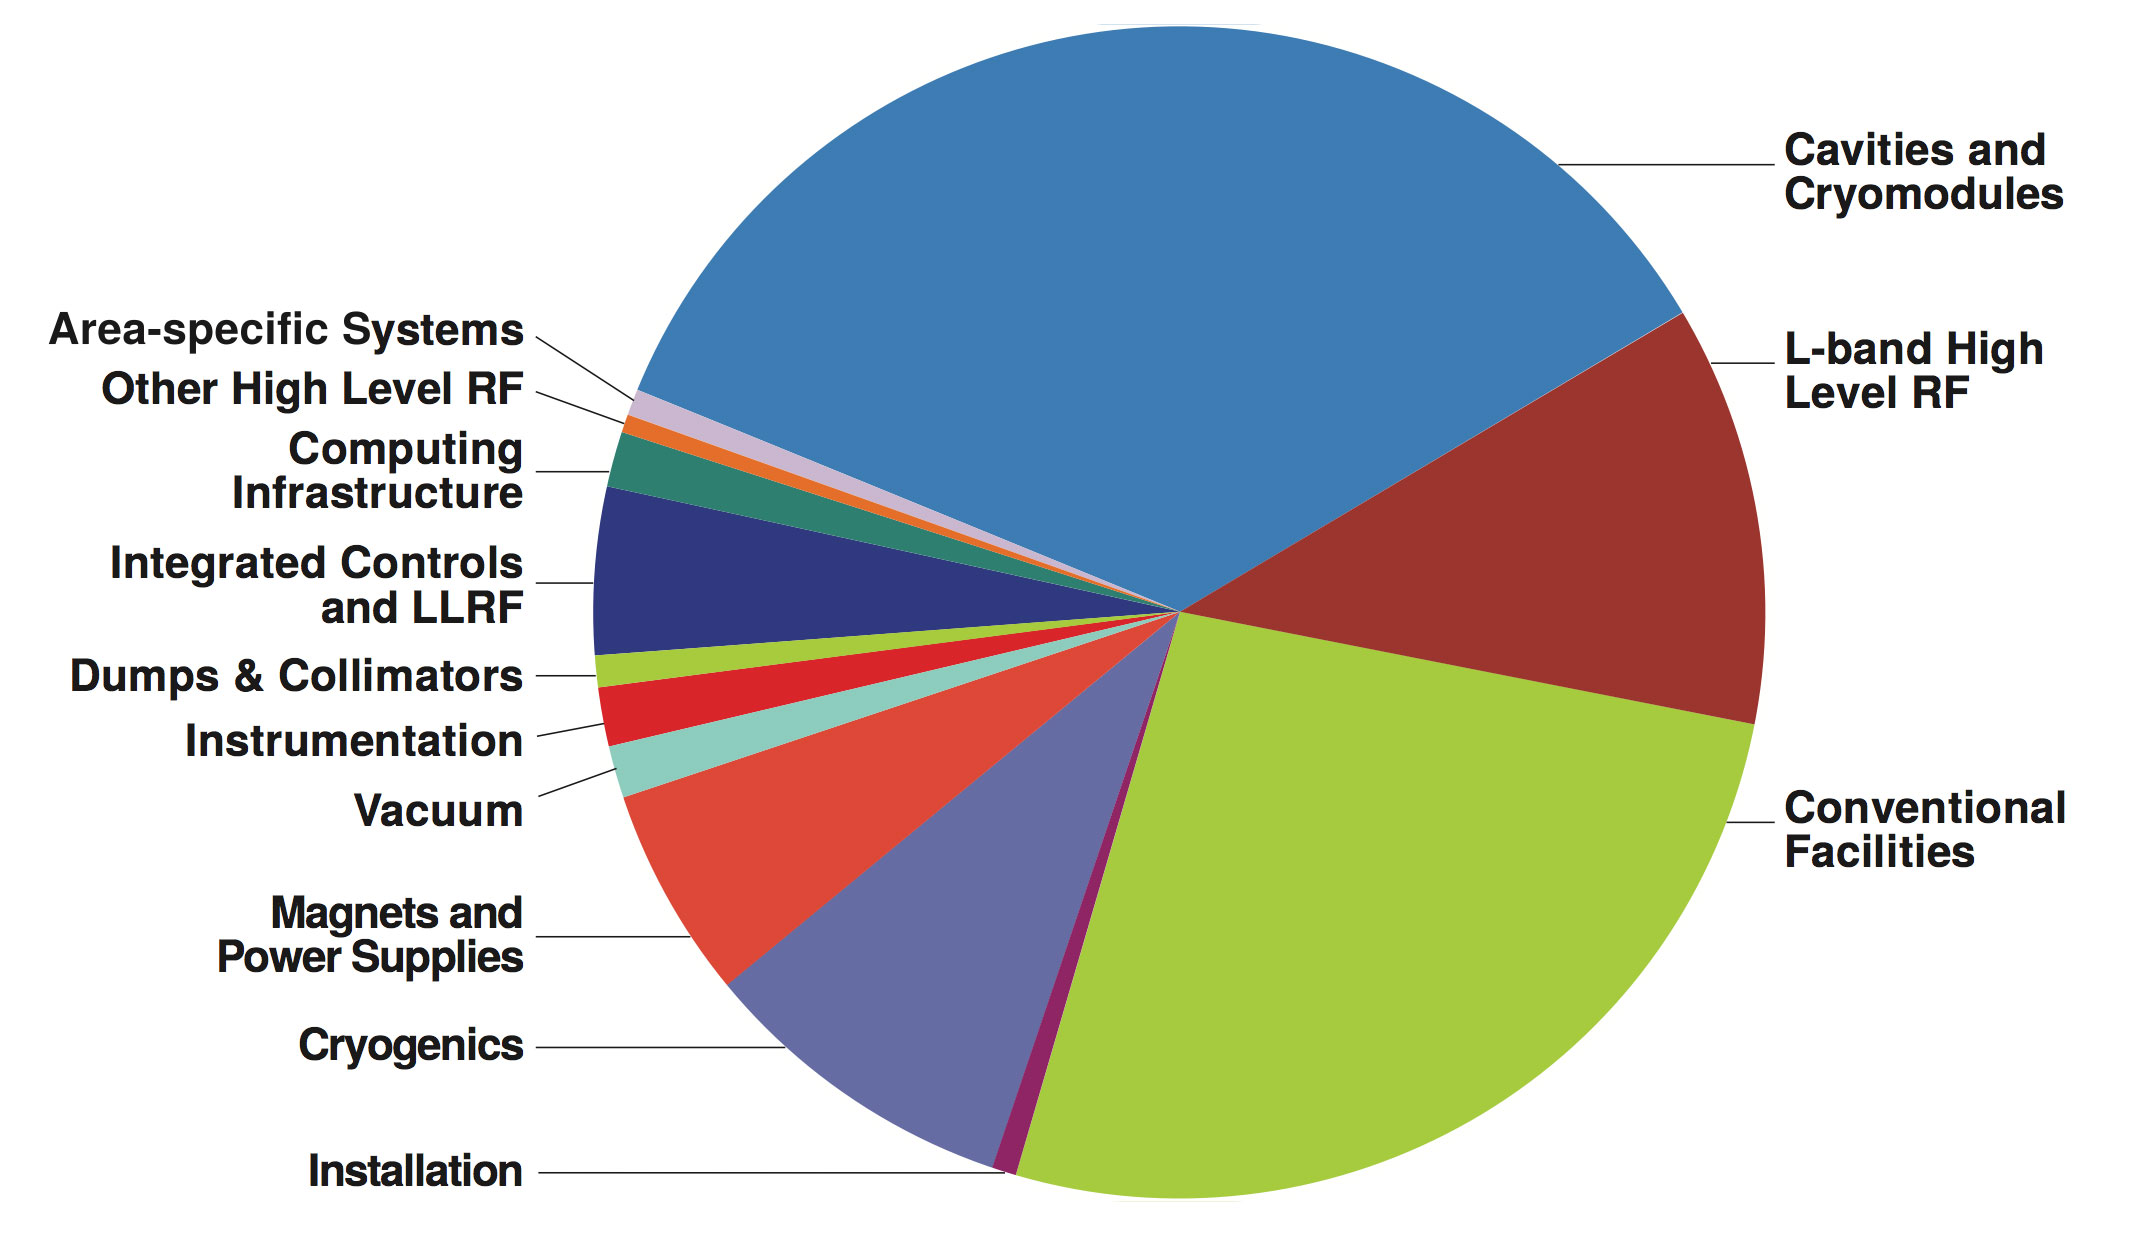
\includegraphics[width=1\textwidth,natwidth=2132,natheight=1246]{ILC_Cost.jpg}
\caption{Sub-system value breakdown \cite{ILC:TechnicalDesignReport}}
\end{figure}
 
The host site geology will determine the most cost-effective tunnelling method approach, while topography can influence the surface structures, access tunnels and shafts. All of these factors can shift the balance of the cost-optimisation and influence the accelerator design. As a result, the final machine will be influenced by the choice of site. In the absence of a definitive site for the ILC, evaluations of different characteristic sites were made. \cite{ILC:TechnicalDesignReport}
 
\subsubsection{Detector costs}

The SiD detector's cost estimate is a construction cost estimate which excludes R\&D, commissioning, operating costs, or physicist salaries. The SiD cost is \$315 million for M\&S, 316 thousand person-hours engineering, 904 thousand person-hours technical, and 51 thousand person-hours administrative labour. The estimated M\&S contingency, reflecting uncertainty in unit costs and some estimate of the maturity of this study, is \$127 million.

The cost of the ILD detector will depend on the option chosen (two options for the vertex detector, which is a multiple layer silicon pixel sensor measuring the position of charged particles, are that it will either consist of 3 double layers or 5 single layers.) and varies between \$350 and \$440 million. This cost does not include labour, or any contingency.
 
\subsubsection{Cost Growth}

Cost growth has been a very common problem for large science projects. For example, the largest such project, the International Space Station, experienced dramatic cost growth throughout the construction, beginning with documented doubling of the construction cost and followed by continuing cost escalation. The reasons are manyfold, but some of them present important lessons for us, like cost growth due to an evolving design, lack of sufficient mechanisms to control cost growth, etc. 

So it is not a complete surprise that a recently finished design review of ITER, a major fusion experiment to be built in Cadarache, France, is forecasting a delay of 1-3 years in its completion date and a roughly 25-30\% increase in its 5-billion (US\$7.8-billion) construction cost. 

Closer to home, the Large Hadron Collider (LHC) also experienced both cost growth and subsequent delays in schedule. The project was originally approved in 1995 for a budget of 2.6 billion Swiss Francs, plus 210 million Swiss Francs for the experiments. The project underwent a major review in 2001, resulting in an increased budget and a delay in the start date from 2005 to 2007. By the time of actual commissioning in 2010, the costs had grown well beyond the original budgets. Problems with magnets were a major contributor, but underestimating the costs when the project was proposed and approved was also a big factor. \cite{ILC:CostMegaprojects}
  
\subsubsection{Construction Cost}

Earlier reports on governance generally favoured a regional approach to funding, e.g. the host region providing 50\% of the overall cost and the non-host regions 25\% each. Developments since the date of these reports increasingly call into question the viability of such models. The rapid industrialisation of in particular China and India and their increasing expenditures on science have changed the face of science in Asia. Japan no longer dominates the scene, although it is still by far the strongest participant in particle physics. Still, both India and China have greatly increased activity. Since, unlike the situation in Europe, there is no strong coordinating institution similar to the EU, it is difficult to see how an Asian contribution to the ILC could be apportioned without complex multilateral negotiations in an undefined forum. Similarly, the relative commitment of the US to particle physics has declined to the extent that it does not seem likely that the Department of Energy would be willing to invest 25\% of the ILC cost in a facility overseas.
 
The 50:25:25 model of regional contributions is more or less a GDP-related model, similar to that used by CERN, though it uses Net National Income (NNI) rather than GDP. A model for the ILC based on that used by CERN could be considered; it has a saturation feature that no one country can contribute more that 25\% of the total CERN budget. Unfortunately as remarked above, it seems unlikely that the US would be willing to contribute 25\% of the project cost, which is the amount that its GDP would dictate under the CERN-like arrangement.
 
All models must include a substantial `host premium' by which the host pays a significantly larger share of the project than would otherwise be expected. This takes into account the very substantial economic benefits which the host area will attain. The size of such a premium should not be fixed to an arbitrary amount, such as 50\%, but instead should be agreed between the major partners at the start of the project.

We conclude that the ILC funding model should be based on a substantial host premium together with a `share model' in which participants contribute an agreed share of the project not just proportional to GDP or other measures of economic wealth.
 
\subsubsection{Running Cost}

The ICFA guidelines in regard to running costs have been modified to permit operating costs to be shared among the project participants. They say it is important not to double count the benefits of hosting, leading to a premium in both construction and running, unless this is really justified by the economic analysis.

The ICFA recommends that running costs should be evaluated at the time of setting up the organisation and a suitable algorithm agreed to. A commonly chosen algorithm is that running costs should be distributed roughly proportional to capital contributions.
 
\subsubsection{Decommissioning Cost}

It will be the responsibility of the state that provided the particular Work Breakdown Structure (WBS) item to decommission it; the host should have enduring responsibility, including if necessary returning the site to the condition before the project was constructed.
    \end{subsection}

    \begin{subsection}{Location \& Governance}
        \subsubsection{A History of Organisational Committees}

The International Committee for Future Accelerators (ICFA) was set up in 1976 to facilitate and encourage international collaboration in all stages of the construction and use of high energy particle accelerators; organising regular world-inclusive meetings to discuss future plans and workshops for progressing the R\&D of the technology required to overcome problems in accelerator development. \cite{ICFA}

Membership of the ICFA is representative of the particle physics activity in the different world regions and is as follows (member numbers are indicated in brackets): CERN member states (3), USA (3), Japan (2), Russia (2), Canada (1), China (1), Other Countries (3) \cite{ICFA}. The members tend to be the directors of the large accelerator laboratories in the world (i.e CERN, Fermilab, IHEP , KEK, DESY and SLAC.) Although the ICFA cannot guarantee the completion of goals, because of its broad international representation, it acts like a ``conscience'' in the particle physics field and its recommendations influence and initiate national activities (the committee has no formal power to cause any resulting action). \cite{ICFA}

The ICFA set up panels for specific technical accelerator and particle physics topics, where expertise beyond that of the ICFA members is required and international discussion is valuable. Each panel composes 16 members representative of the world regions. One of these panels is the ``International Linear Collider Steering Committee'' (ILCSC) set up in 2002 to promote the construction of an Electron-Positron Linear Collider through a global collaboration focusing on science, technology, outreach and organisation of the Linear Collider project. \cite{ICFA}

The ILCSC set up a Parameters Subcommittee for the ILC to obtain a worldwide consensus on the parameters for the machine and also set up the International Technology Recommendation Panel (ITRP) which in 2004 recommended basing the ILC main LINAC design on superconducting radio frequency (SCRF) technology \cite{Funding:Interactions:ICFAPress}. The ILCSC established the Global Design Effort (GDE) in March 2005 to co-ordinate the global R\&D and technical design of the ILC, and appointed Barry Barish as its current Director reporting to the ILCSC.

On February 21st 2013, the two most mature future particle physics projects \textendash ILC and CLIC \textendash united, forming an official organisational partnership called the ``Linear Collider Collaboration'' (LCC) which will continue to advance the global development efforts for the next linear collider. \cite{LCC:Press1} Following the completion of the ILC TDR by the GDE in June 2013, the ILSC went out of existence and was replaced by the ``Linear Collider Board'' which will oversee activities of the LCC.

ILC and CLIC have similar goals but they use different technologies and are at different development stages. Therefore the LCC is split into three main research sections; ILC section, CLIC section and a section for physics and detectors. For the ILC, the main focus is preparing it for possible construction while also advancing acceleration technologies and design optimisation. For CLIC, research into the novel drive beam acceleration concept continues to be advanced.  For Physics and Detectors, R\&D of new detector technologies and concepts continues, fully exploiting the synergies that exist between ILC and CLIC detector requirements. \cite{LCC:Press1}

The ICFA has no funding, even for the R\&D. In 2003, a group of representatives from funding agencies and governments around the world formed the ``Funding Agencies for Large Colliders'' (FALC) to help develop international funding mechanisms for the next international large collider. Meetings take place twice a year where the progress of global R\&D and the status of future large colliders and detectors are discussed; meetings are attended by chairs of the ICFA, LCB and LCC. The next meeting will take place in May 2014 \cite{Funding:FALC:History}. Although FALC is an informal group, it helps coordinate an international dialogue to prepare the necessary financial arrangements for the next particle accelerator which will cost more than one nation or one region can afford \cite{Funding:FALC:Report}.

\subsubsection{Project Implementation and Governance}

When large scale research endeavours go beyond what a single nation or region can sustain, its guiding principles must expand. A central principle is ``openness to the world''. High energy physics (HEP) has been international in nature since the beginning. Its mission has been to explain the fundamental laws of nature and the universe with resulting discoveries naturally deemed to be common assets of all people everywhere. The basic principle is that HEP ``should be pursued independently of any political, national, ethnic, or other constraints'' \cite{ILC:PIPReport}.

The next international project (be it ILC or CLIC) will be a unique opportunity to demonstrate internationalisation and political cooperation on a global scale in particle physics which will result in many positive consequences for technology, science and education. This is an important way in which the next particle collider will make a valuable global contribution.

The governance of such a large international project will be complex and strong host laboratory will be essential. The location of the collider determines the host and host responsibilities include: providing services necessary for a world-class research facility (i.e. transport links, housing, social facilities) and making the necessary contributions to the infrastructure, construction and operations. Additionally it will need to prepare for legal status as an international organisation with tax exempt status. It would be an advantage for the host to have a major national laboratory nearby to strengthen the project through a cooperative relationship.

The ILC currently has no ``host laboratory'' however the location is due to be finalised by 2015 with Japan the main contender. Japan ticks all the boxes in terms of providing a strong host: financial stability, good transport links and social facilities able to support the large influx of people, the total population of the researchers, lab employees and their families will be $\sim$10,000 people. Also Japan has a major laboratory, KEK, whose main function is to provide the particle accelerators and other infrastructure needed for HEP. KEK has been playing a lead role in R\&D efforts for the ILC, hence if Japan hosts the project, it will be greatly strengthened by this synergistic relationship. Furthermore on 6th February 2014, KEK announced the creation of an office responsible for the ILC project, the ``ILC Planning Office''. The new office will coordinate and integrate efforts on planning, scheduling and managing research activities. This new office is a starting point and is planned to be expanded into an international ILC pre-laboratory. \cite{LCC:Press2}

CLIC on the other hand is likely to be hosted at CERN (according to the conceptual design report) which gives it many advantages in terms of existing social facilities and infrastructure at the site.

\paragraph{Governance Model Proposed for the ILC.}

Governance involves defining all the distinct elements required to set up a good ILC organisation with clear aims, good management and supportive governments and funding agencies. Because the ILC is an unprecedented project, ``prescriptive'' governance methods from previous international projects cannot simply be applied. Instead, the approach to governance on previous international projects \textendash ALMA, ESS, FAIR, ITER, LHC, SKA and XFEL \textendash was extensively compared and information organised into pro-formas, each with a recommended solution for the ILC as follows: \cite{ILC:PIPReport}

\begin{enumerate}

\item Legal status: ILC should be set up as an international treaty organisation (similar to ITER). An important part of the treaty will be to guarantee access to the ILC lab to all interested parties.

\item Management structure: ILC should have a strong council representing member states, a Director General (DG) and a Directorate. The DG should have authority from the Council to make timely decisions without the need to refer back to Council. A project team will be responsible for the final site-dependent technical design, component specifications, installation, commissioning, maintaining schedule and the common fund. They will report to the ILC council.

\item Representation and voting structure in the governing body: each Council member state will have 2 delegates – one representing the government, the other a particle physicist \textendash and a maximum of 2 advisors (modelled on CERN). The Council will decide non-financial questions by simple majority and financial questions by a majority of financial contributions plus a majority of individual member states.

\item Duration of the ILC agreement: the ILC agreement will be fixed term - a construction period of $\sim$8 years plus 20 years of operation including the 1TeV upgrade; it should be extendable on council agreement in periods of five years. Stable membership is important in international organisations in order to plan sensibly, therefore withdrawal will not be allowed until a minimum of ten years after the agreement comes into force and then only after one year's notice of withdrawal.

\item Attribution of in-kind contributions and value engineering: the construction project will be based on a work breakdown structure (WBS) system (this is standard in all major projects). The majority of contributions to the project's infrastructure will take the form of in-kind contributions from member states. Value engineering will be used to optimise the performance/cost ratio of each WBS item in order to determine its financial contribution size. It is vital to have an adequate common fund (of at least 20\% financed by cash of member states) to give management flexibility i.e. WBS elements that don't come from in-kind contributions like installation costs will be supported by the project common fund.

\item There should be a central contingency budget with a maximum of 10\% of the total project cost, to be released as appropriate by the Council. Depletion of the central contingency will initiate appropriate descoping of the project, decided by management with Council's agreement. The ability to descope assures governments that the ILC project will not spiral into major cost overruns. The most obvious method of descoping is to reduce the energy reach of the machine by installing fewer superconducting cavities.

\item Running costs and decommissioning: running costs will be distributed approximately proportional to state capital contributions. Decommissioning of a WBS item will be the responsibility of the state that provided it. The Host State will have residual responsibility.

\item Budgetary and personnel policy: the lifetime of the ILC lab is a fixed term and likely to be shorter than the careers of its staff, therefore a personnel policy using ``seconded personnel from participating institutions'' is recommended. This policy avoids a potential imbalance in the expert population that could result when participating organisations lose too many staff or from the surplus of experts after ILC's completion if a ``direct employment'' policy was used.

\end{enumerate}

\paragraph{CLIC/ILC Governance Comparison.}

The ILC governance model is taken from the completed ``Project Implementation Plan'' (PIP) of the ILC. CLIC on the other hand doesn't have a PIP (due to begin the PIP in 2017); however as CLIC is also being realised as a global collaboration, it is likely to be modelled on a similar governance structure with the pro-formas described above.

CLIC was originally a CERN project and has developed into an international collaboration comprising over 70 institutes in 30 countries \cite{CLIC:Organisation}, however it is still mainly centred at CERN; the CLIC test facility (CTF3) was built at CERN by an international collaboration to demonstrate CLIC's feasibility. ILC has been a global program from the outset whose governance and technological endeavour is shared across multiple laboratories and regions; nearly 300 laboratories and universities from 35 countries are involved in the project \cite{ILC:Collab}.

\subsubsection{Location}

The landscape and geology of a site will influence the machine design i.e. the tunnel alignment, tunnel depth and tunnel access will vary at different sites, therefore it will be necessary to modify the original generic design of each collider to produce a site-dependent design.

\paragraph{ILC Location.}

The ILC footprint requires the site to be 50 km long (to accommodate the planned machine upgrade to 1TeV) and a maximum width of 1km for accommodating the central interaction region and adjacent damping ring. Positioning of conventional and technical machine support facilities will vary for different sites. For relatively flat terrain, allowing for vertical access shafts to the tunnel complex below ground, these facilities will be housed on the surface. In mountainous regions which use horizontal access to the tunnel complex, underground caverns may be used to house some or all of the support equipment. \cite{ILC:PIPReport}

Different characteristic sites were evaluated in the TDR which lead to two different methods of transporting the RF microwave power to the accelerating structures: one suitable for a flatter terrain using the Klystron Cluster Scheme (KCS), and one for a more mountainous terrain \textendash the Distributed Klystron Scheme (DKS). \cite{ILC:TechnicalDesignReport}

The $e^-$ and $e^+$ main linac portions of the ILC can be constructed in an enclosure following the Earth's curvature. However the system delivering beams to the interaction region must be constructed in a laser straight enclosure. All sample sites considered in the ILC's TDR positioned the $e^-$ and $e^+$ main linacs and beam delivery system in stable rock geology at a minimum depth of 100m for relatively flat terrain and at even greater depths in mountainous terrain. Considering the minimum depth required for shielding radiation purposes is 8m, it is very safe \cite{ILC:PIPReport}.

The ILC will place a considerable additional demand on the capacity of regional utility infrastructures; for example electrical power requirements will be 250-300MW. To accommodate the increase in local population, the capacity of support utilities i.e. electrical power distribution, waste disposal systems and fuel resources such as oil and gas, will need to be reviewed. Existing rail access to a proposed ILC site would be beneficial. Since a significant amount of equipment will be shipped in from many different locations, convenient access to a seaport, airport and highways capable of supporting loads of up to 50 tonnes to the site is desired. There will be a constant flux of personnel so easy access to an international airport is essential.

Proposed host countries for the ILC are Japan, Europe (CERN) and the USA (Fermilab). In the USA, the proposed site near Fermilab is relatively flat and will have about one quarter of the machine on the Fermilab site with the tunnels bored into adjoining dolomite rock 30 \textendash 100 m below the surface. There are two possible ILC sites in Asia: Kitakami in northern Japan and Sefuri in the south. Both sites have uniform terrain located along a mountain range and tunnel depth will range from 40 \textendash 600 m in uniform granite geology well suited to modern tunnelling methods. The European site is located at CERN (Switzerland) and runs parallel to the Jura mountain range, close to the CERN site, mostly in molasse rock with a typical depth of 370 m. \cite{ILC:TechnicalDesignReport}

The International Linear Collider Committee of Japan evaluated the Kitakami site to be the best location for the ILC in Japan on August 23, 2013 \cite{LCC:Press3}. The Kitakami site has geological advantages such as stability against earthquakes; despite its proximity to the 2011 earthquake epicentre, the area was naturally protected by the mountains and rock geology as the rocks were not bent but moved together \cite{Japan}. Underground facilitates also sustain less seismic damage than surface structures. The committee concluded that the site would be able to accommodate a seismic resistant design able to withstand earthquakes larger than magnitude 9.0. Another geological advantage of the Kitakami site is its water drainage, which lowers the risk of a potential extension to the construction period. The estimated total length of the access tunnels was evaluated to be shorter at Kitakami hence reduced tunnelling costs. In addition \cite{ILC:FundingAgencies} the Kitakami site provides a good environment for living and research and is located near the Shinkansen railway line which can reach Tokyo in just 2 hours, and the nearest major city Sendai, is only a 10 min train ride away.

\paragraph{CLIC Location.}

Key features of the CLIC layout are: the laser straight tunnels following the Earth's curvature (unlike the ILC), access shafts and surface installations approximately every 5 km and the main linac to be housed within a single tunnel with an internal diameter of 5.6 m. The 500 GeV machine will have a site length of 17.74 km and the upgraded 3 TeV has a machine length of 49.28 km. \cite{CLIC:Concept}

The proposed location for CLIC is in Geneva near CERN. The $\sim$50 km long 3 TeV machine will lie on the French \textendash Swiss border, with the interaction region located in the Prevessin campus in CERN. The CLIC site will be between the high mountains of the Alps and the lower mountain chain of the Jura. Geneva has excellent transport and communication networks since it is already home to many international organisations. There are direct links to Geneva airport which is just 5 km from CERN. The governments of France and Switzerland have long standing agreements concerning the support of particle accelerators in the Geneva regions, making it very likely that the land could be made available free of charge, as it was for previous CERN projects. Also the CERN area has very stable and well understood ground conditions with up to date geological records, from the civil engineering works for the LHC, which will be used for CLIC to minimise the costs and risk to the project.

The physical positioning of CLIC was developed so that as much underground volume as possible would be contained in the molasses rock with any known geological faults or environmentally sensitive areas being avoided. Also it is anticipated that the central injection complex and interaction region will be built on the at the Prevessin campus, CERN.

The tunnel will be constructed mostly in stable molasse rock at a depth of 100 \textendash 150 m in an area with little seismic activity. In especially sensitive areas or areas where the shafts are very deep (several hundred metres), inclined access tunnels are foreseen. When the tunnel or access shaft passes through areas with potential water entry, special excavation techniques like ground freezing is used. Ground freezing involves freezing the ground with a primary cooling circuit using ammonia and a secondary circuit using brine at -23ᵒC in vertical tubes in holes 1.5 m apart.

\begin{figure}[!htb]
\centering
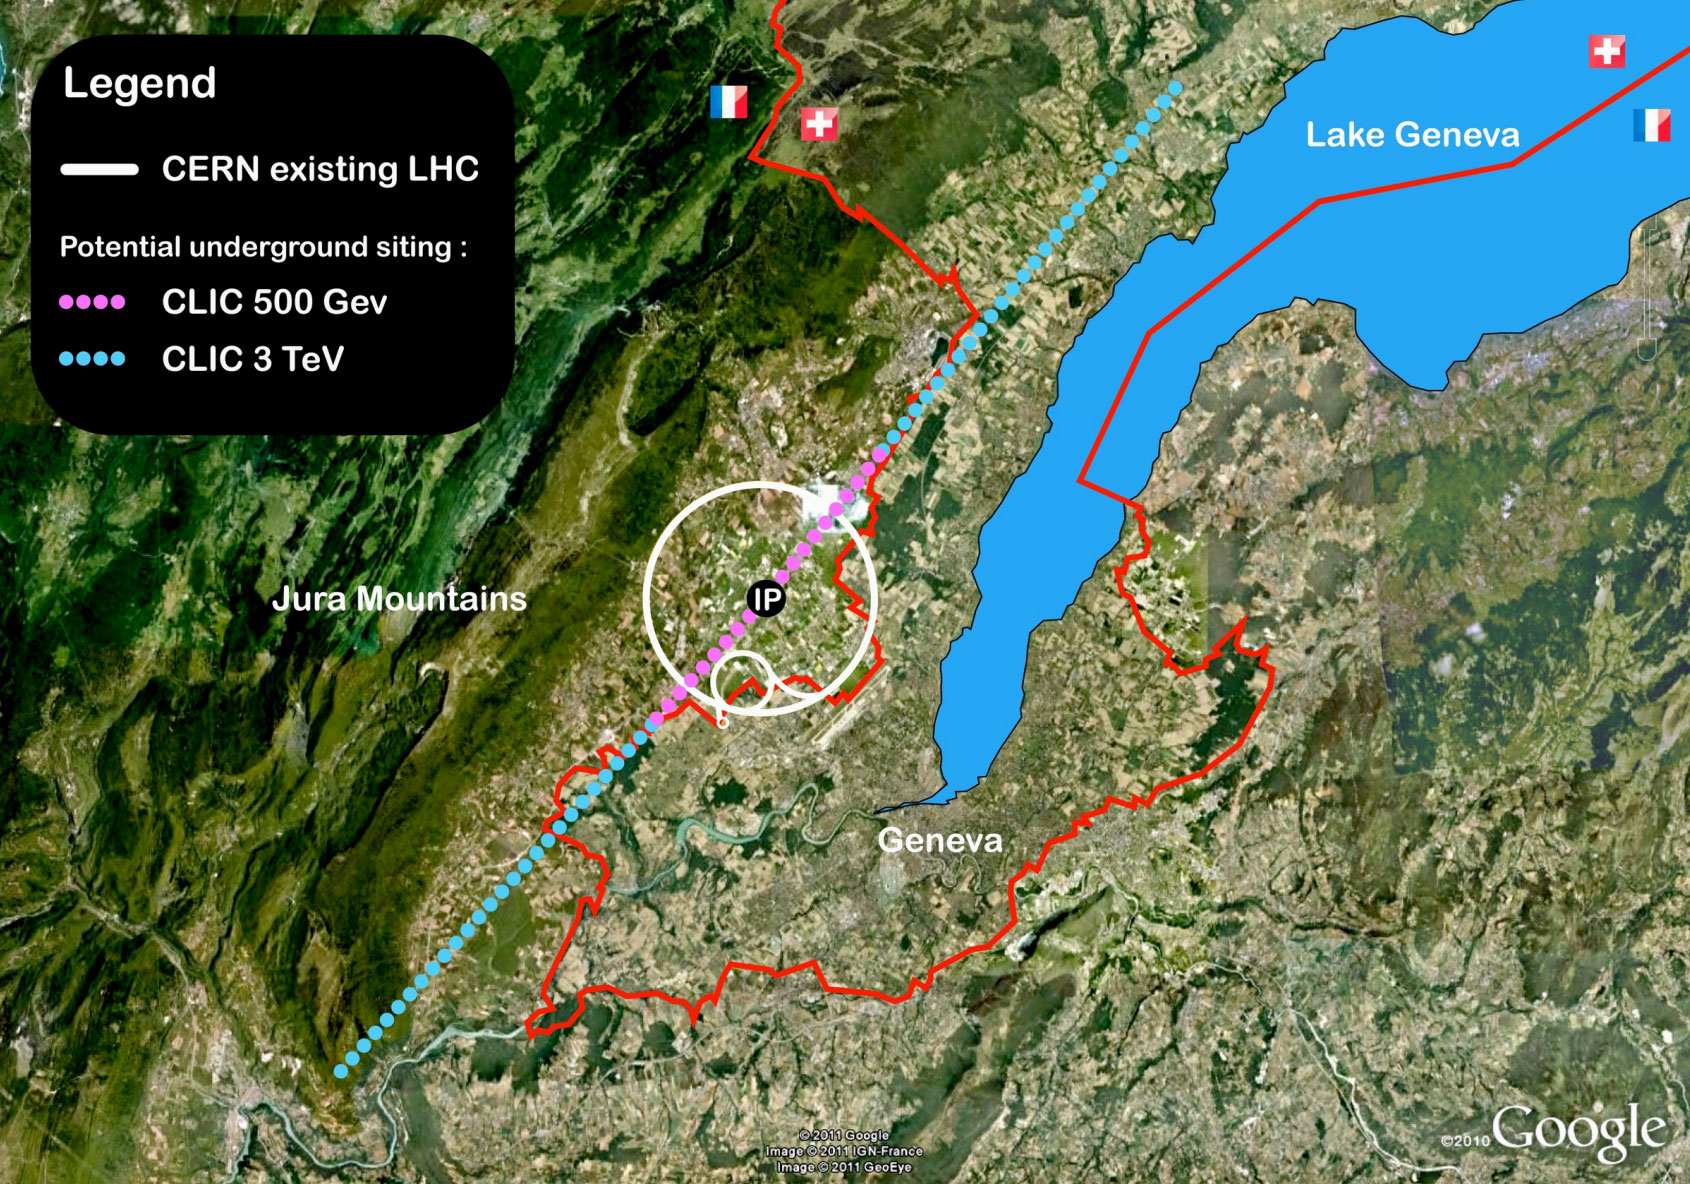
\includegraphics[width=1\textwidth,natwidth=1690,natheight=1184]{CLIC_Map.jpg}
\caption{Map Showing Potential Location for CLIC Accelerator Complex \cite{CLIC:Concept}}
\end{figure}

\paragraph{ILC/CLIC Location Comparison.}

The proposed locations for ILC and CLIC are shown to be feasible. However while the potential location for CLIC is merely conceptual, a great deal of research has gone into selecting the location for the ILC with a detailed analysis of potential sites.

The 2008 economic crisis led the US and UK to cut funds to the collider project and after the Great East Japan earthquake of 2011, Japan had an excess of reconstruction money which could be used for the ILC project indicating that Japan is most likely to host the ILC. In this case, the ILC will be located at Kitakami which has been shown to have geological advantages for construction and capable of providing good social facilities and transport links required. It would not make sense to build the ILC at CERN because CERNs priority for the next 20 years will be in exploiting the LHC at the higher energy range of 14 TeV. Also, it will be of international benefit to spread particle physics facilities across the world. Given the current economic climate of Europe, and the fact that Japan has offered to fund 50\% of the material costs of the ILC, Japan looks like the most likely location.
 
 
\subsubsection{Politics and Economics}

The construction of the next particle collider will depend on political decisions and the recognition of governments to fund it. Therefore it is important for governments to be involved as actively as possible and be kept informed of the project progress via FALC. However, scientific and political aspects of the project must be separated. While decisions regarding legal agreements, budget allocation and site selection for the next linear collider will be made by government agencies of participating nations, it is important that technical outlines and specifications are protected from any political compromises and are based solely on scientific facts. \cite{ILC:PIPReport}

For the ILC, the host country won't be finalised until around 2015 but with the current economic climate of Europe and the US, an international consensus is rapidly forming that Japan is will host for the ILC. The global recession has meant that even the money needed for R\&D to finalise the design was tight \cite{Funding:Nature}.  With the estimated cost of \$7.8billion, the project has struggled to gain support from governments however the Japanese government has proposed to fund 50\% of the material costs, though the project will need international commitment in order to move forward.

Japan lost out in hosting the fusion reactor ITER in 2005 to France and has been looking for a world-class international science project since. The 2011 earthquake and tsunami in Japan gave rise to an excess of reconstruction funding, some of which could go towards a scientific project such as the ILC. The ILC has broad political backing in Japan with high profile politicians across the political parties supporting the project. This shows Japan's desire to play a more collaborative role in the global scientific community. \cite{Funding:NaturePress1}

The Japanese government budget proposal for the 2014 fiscal year includes an official budget for the ILC. Although a small amount,   $\sim$\$500k, it shows that the ILC is a recognised project of the Japanese government and is also the first official national budget for the ILC. The budget will be used to make a detailed study of the feasibility of an international framework for the ILC as a global project, as only after establishing international partnerships will Japan take the project further. \cite{LCC:Press4}
 
Currently the situation outside of Japan is as follows: countries are being contacted by Japanese government representatives to discuss possible contributions and a view of the ILC to be hosted in Japan has been integrated into the 2013 update of the EU strategy for HEP. If the ILC is approved in Japan, Europe will make a contribution. The US may be more reluctant to participate due to current budgetary constraints but the international diplomacy features of the project are sure to attract the US government's interest; a recent critical step is the positive inclusion of the ILC project in the US strategy for HEP \cite{Funding:NaturePress1, LCC:Press5}.
 
The ILC is more politically advanced in terms of attracting interest amongst governments compared to CLIC which doesn't yet have a technical design report or project implementation plan.
 
As well as the prestige of hosting a world-class science project, there will be long term economic benefits to the hosting region. The Japanese Productivity Centre calculated that the ILC could have a financial impact of over \$40 billion over a 30-year period and create 250,000 direct and indirect jobs \cite{Funding:SwissInfo}. The ILC facility will attract new businesses, for example, the technology spinoffs, which will boost the local and regional economies. No figures are available for CLIC but the economic benefits will be similar to ILC.
    \end{subsection}
     
 \end{section}
 
 \begin{section}{Conclusion}
 
     In conclusion, we have chosen ILC as the next future collider. We feel that it is the best option as it combines both feasibility in terms of location, cost and technology, and physics reach.

\subsection{Location}

The proposed location of CLIC was CERN, whereas ILC's main contender for location is in Japan. A concern for our group was that if a new collider was to be built at CERN, its energy budget would have to be expanded to accommodate this. CERN already has an infrastructure, in contrast to ILC where infrastructure would need to be created. However plenty of research has been carried out to ensure that Kitakami in northern Japan, the chosen location for ILC, is safe, including topography, geology, drainage and earthquake studies, as well as examining transport links and nearby major cities.

\subsection{Finance}

In terms of finance, ILC has a highly developed financial plan, while CLIC's funding model is not finalised and is currently inaccessible. The cost of ILC has been estimated at \$7.8 bn. As the research has been carried out into the exact costs of ILC and a sub-system value breakdown has been given, this estimate is more reliable than the estimates of \$6 billion found for CLIC.

\subsection{Spin Offs}

The spin offs that both particle accelerators would lead to are very similar. From improved medical linear acceleration, smaller beam radius for radiotherapy uses and even nuclear waste disposal, both accelerators would achieve these aims. Due to CLIC's higher acceleration gradient, power consumption and the size of the equipment for hospital linear accelerators could be greatly reduced. However, there is no evidence to suggest that this would not be the case for ILC. In addition, because ILC could be built within a shorter timescale, it could have the added spin off of attracting people and skills to the area where the accelerator is built, and ensuring the international community of scientists is pushed forward.

\subsection{Energy Reach}

CLIC undeniably has a higher energy reach than ILC: 3TeV in comparison to 1TeV. However, the question we found ourselves asking was, ``is this higher energy necessary?''  One argument was that pushing the energy frontier is always desirable, yet the evidence for particles at higher energies was lacking at best. For instance, both CLIC and ILC had goals of discovering supersymmetric particles. However, the existence of supersymmetry is doubtful and is becoming increasingly unlikely. In addition, LHC has not found any evidence of supersymmetry at higher energies which we feel would be needed to justify the higher energy range of CLIC. ILC seems to have a clear science goal which is not the case for CLIC. It would be hard to galvanise a project such as CLIC where its aims may not be achievable. We found that the risk of committing to a large scale project such as CLIC with no little evidence of the particles the higher energy could be used to investigate, was not attractive.

\subsection{Feasibility}

Both ILC and CLIC could be used to probe Higgs in more detail, therefore due to the higher feasibility of the former, it seems as though ILC is the clear choice.

The LCC is currently focusing on possible construction for ILC, in comparison to the focus on research for CLIC. Therefore in the international physics community ILC is already seen as closer to construction, and more feasible than CLIC. CLIC still needs the technology for its two beam linear accelerators and low beam emittance to progress before construction can occur, although these are in their final stages of development. Instead of waiting for the technology and high acceleration gradient to be developed for CLIC, we have decided to ride the momentum of the LHC's Higgs discovery and keep the next generation of physicists engaged by building ILC. With the cleaner collisions of a lepton collider in comparison to LHC, the Higgs can be probed sooner rather than later by deciding on ILC, which will galvanise current interest in the Higgs boson in the scientific community and in the press.
 
 \end{section}
 
 \clearpage
 \hfuzz = 1000pt
 \printbibliography
 
 \clearpage
 
 \appendix
 \begin{section}{Tables}
    \label{appendix:tables}
    \begin{sidewaystable}[!htb]
\begin{tabularx}{\textwidth}{X | X | X | X | X}
    \textbf{Parameter}                     & \textbf{CLIC Nominal}          & \textbf{2011}                                              & \textbf{2012}                                       & \textbf{2013}                     \\ \hline
        $I_{initial} (A)$             & 4.2                   & 7                                                 & -                                          & -                        \\
        $I_{final} (A)$               & 100                   & 28                                                & 30                                         & -                        \\
        $Q_b$                         & 8.4                   & 4 (2.3 nom.)                                      & -                                          & -                        \\
        Norm. Emittance RMS (mm)      & $\leq$ 150            & 150 (factor 4 comb. beam, vertical)               & $\leq$ 150 (factor 8 comb. beam, vertical) & -                        \\
        Bunch Length (mm)             & $\leq$ 1              & $\leq$ 1 (linac), $\leq$ 2 (CLEX)                 & $\leq$ 1 (CLEX)                            & -                        \\
        E (GeV)                       & 2.4                   & 0.12                                              & -                                          & 0.15                     \\
        $T_{pulse}$ initial ($\mu s$) & 140                   & 1.4                                               & -                                          & -                        \\
        $T_{pulse}$ final ($ns$)      & 240                   & 140 (240)                                         & 140 (240)                                  & 140 (240)                \\
        Beam Load Eff. (\%)           & 97                    & 95                                                & -                                          & -                        \\
        Deceleration (\%)             & 90                    & 26                                                & 35                                         & $\geq$ 50                \\
        Phase Stability at 12GHz      & 0.2                   & -                                                 & 0.5                                        & 1                        \\
        Intensity Stability           & $0.75 \times 10^{-3}$ & $0.5 \times 10^{-3}$ (linac), $10^{-3}$ (comb. 4) & $2 \times 10^{-3}$ (comb. 8)               & $\leq 10^{-3}$ (comb. 8) \\
\end{tabularx}
    \caption{Major parameters at the CTF3 facility, as compared to CLIC nominal values. The goal values of the parameters are also included. (CLEX – CLIC Experimental Area) \cite{CLIC:Concept}}
\label{tab:CLIC:Feasi1}
\end{sidewaystable}

\clearpage
 
 \end{section}
 
 \begin{section}{Interviews}
     \subsection{Prof. Jon Butterworth, 17/02/2014. Mary O'Donnell \& Harapan Ong} 
\label{interview:butterworth}

\subsection{Prof. Robert Thorne, 08/02/2014. Mary O'Donnell \& Harapan Ong}
\label{interview:thorne}

\subsection{Prof. ?? Waters, ??/02/2014. Mary O'Donnell \& Harapan Ong}
\label{interview:waters}
 \end{section}

 
\end{document}
